%===============================================================================
% Brno University of Technology
% Faculty of Information Technology
% Academic year: 2018/2019
% Bachelor thesis: Monitoring Pedestrian by Drone
% Author: Vladimir Dusek
%===============================================================================

\chapter{Trénování detektoru}
\label{chap_4}

Při trénování neuronových sítí probíhá spoustu relativně snadných výpočtů. Například aplikace konvolučních filtrů na vstupní obraz nebo výpočet podvzorkování v~pooling vrstvách. Tyto jednotlivé výpočty jsou na sobě vzájemně nezávislé, proto mohou být prováděny paralelně. Doba trénování tedy může být mnohonásobně urychlena použitím grafických karet, které mají běžně tisíce jader.

Využitá knihovna Tensorflow podporuje akcelaraci pomocí grafických karet s~podporou architektury CUDA (Compute Unified Device Architecture)~\cite{docsCuda}. Jedná se o~platformu pro urychlení výpočetně náročných úloh. Typicky takových, kde je možnost snadno využít paralelizaci. Použití této architektury je omezeno pouze na grafické akcelerátory a výpočetní karty společnosti nVIDIA, která ji vyvíjí.

Pro účely hlubokého učení stojí nad architekturou CUDA ještě knihovna cuDNN (CUDA Deep Neural Network library)~\cite{docsCuda}. Ta poskytuje vysoce vyladěné implementace pro standardní úlohy, jako jsou konvoluce, podvzorkování, normalizace a aktivace vrstev. Toto API pak už přímo využívají vývojáři knihoven pro hluboké učení a odprošťuje je od ladění nízkoúrovňového výkonu GPU.

Samotné trénování pak probíhalo na stolním počítači s~grafickou kartou nVIDIA GeForce GTX~1070, která má 1920~CUDA jader. Bylo nutné manuálně doinstalovat veškeré závislosti varianty Tensorflow využívající GPU akceleraci. Fizyr RetinaNet vyžaduje knihovnu Keras verze~2.2.4, ta je součástí až Tensorflow~1.13. Tato verze Tensorflow podporuje pouze CUDA~10.0 a cuDNN~7.4.1, případně novější. CUDA~10.0 požaduje ovladač grafické karty verze alespoň~410. Bylo nutné vše podřídit těmto závislostem. Po jejich úspěšném nainstalování bylo trénování realizováno na čisté instalaci Ubuntu~18.04 s~ovladačem GPU~418.43, CUDA~10.0 a cuDNN~7.4.2.

%===============================================================================

\section{Implementace detektoru}
\label{sec_retinanet_implementation}

Jak bylo vysvětleno v~sekci~\ref{sec_detection_networks} detekční síť RetinaNet se ukázala vhodná pro účely této práce. Zvolil jsem implementaci od společnosti Fizyr.\footnote{Github repozitář Fizyr RetinaNet je dostupný na \url{https://github.com/fizyr/keras-retinanet}} Jedná se o~nizozemskou firmu, která se specializuje na vytváření software v~oblasti hlubokého učení. Implementace je \textit{open-source} a je veřejně přístupná na repozitáři GitHub. Síť je napsána v~jazyce Python pomocí knihovny Keras v~její nejnovější verzi~2.2.4 využívající knihovnu Tensorflow jako \textit{backend}. Keras poskytuje vysokoúrovňové rozhraní pro rychlé a pohodlné vytváření vlastních modelů neuronových sítí. Další výhodou knihovny je, že nabízí jednotné rozhraní pro práci s~různými \textit{backend} knihovnami z~oblasti strojového učení. V~současné době je to kromě již zmíněného Tensorflow od Googlu také Theano, vyvíjené na univerzitě v~Montrealu a Microsoft Cognitive Toolkit.

Předtrénované modely sítě RetinaNet jsou schopné rozpoznávat kolem 80~různých tříd objektů. Je mezi nimi samozřejmě i člověk. Experimentování ale potvrdilo předpoklad, že z~pohledu ze shora síť chodce spolehlivě nerozezná, ani nedetekuje jako žádný jiný objekt. Proto bylo nutné opatřit vhodný dataset a natrénovat vlastní model.

%===============================================================================

\section{Dataset}
\label{sec_dataset}

Typický záběr monitorování oblasti dronem, kde se mohou nacházat lidé, je z~výšky z~pohledu ze shora. Proto pro úspěšné natrénování modelu bylo potřeba obstarat dataset obsahující záběry z~tohoto pohledu a souřadnice ohraničující pozici člověka ve snímku (anotovaný dataset).

Na klasických uložištích datasetů, jako jsou například Google Open Images, Kaggle, Pascal VOC (The PASCAL Visual Object Classes) nebo COCO (Common Objects in Context), je velké množství datasetů různých kategorií. Ačkoliv dat zachycujících člověka je mnoho, nepodařilo se mi najít žádnou specifickou kategorii pro rozpoznání člověka z~výšky. Bylo proto nutné hledat jiný zdroj.

Stanford Drone Dataset (dále už jenom SDD) je dataset záběrů frekventovaných míst univerzitního kampusu na americké univerzitě ve Stanfordu.\footnote{Stanford Drone Dataset je dostupný na \url{http://cvgl.stanford.edu/projects/uav_data}} Dataset vznikl v~rámci práce \textit{Learning Social Etiquette: Human Trajectory Understanding in Crowded Scenes}~\cite{paperSDD}, která se zabývá analýzou a předpovídáním pohybů nejenom chodců, ale i cyklistů, aut, autobusů apod.

Dataset obsahuje videozáznamy ve formátu mp4 z~8 různých lokací o~celkové velikosti~72\,GiB. Každému videozáznamu přísluší anotační textový soubor, kde je zaznamenána poloha objektů na každém snímku videa. Druhy zaznamenávaných objektů jsou chodec, cyklista, člověk na skateboardu, auto, autobus a golfový vozík. Každá anotace také obsahuje tři příznaky: \textit{lost}, \textit{occluded} a \textit{generated}. Příznak \textit{lost} je zde z~důvodu, pro který byl dataset vytvářen~--~predikce pohybu cíle. Značí, zda se objekt nachází mimo zaznamenávaný obraz. Tedy cíl se objeví v~zaznamenávané ploše, a když ji opustí, je odhadováno kudy se mohl pohybovat dále. Příznak \textit{occluded} značí, že něco objekt překrývá směrem ke kameře. Například chodec zašel pod strom a není na kameře vidět. A~\textit{generated} říká, zda byla anotace automaticky interpolována. Některé anotace byly tvořeny manuálně, zbylé byly vygenerovány (většina).

Použitá implementace RetinaNet zahrnuje trénovací skript \path{retinanet-train} pro doučení vlastního modelu. Skript umí formáty anotací největších skladišť datasetů. Zvolený dataset pro trénování však žádné z~nich neodpovídá. Vlastní anotace je třeba skriptům předat ve formátu CSV a tvaru \path{path_to_image,x1,y1,x2,y2,class_name}. Z~charakteristiky datasetu SDD a zvolené implementace sítě vyplývá, že pro účely této práce bude muset být dataset upraven. A~to jak samotná trénovací data tak anotace.

\begin{figure}[H]
    \centering
    \begin{minipage}{.5\textwidth}
        \centering
        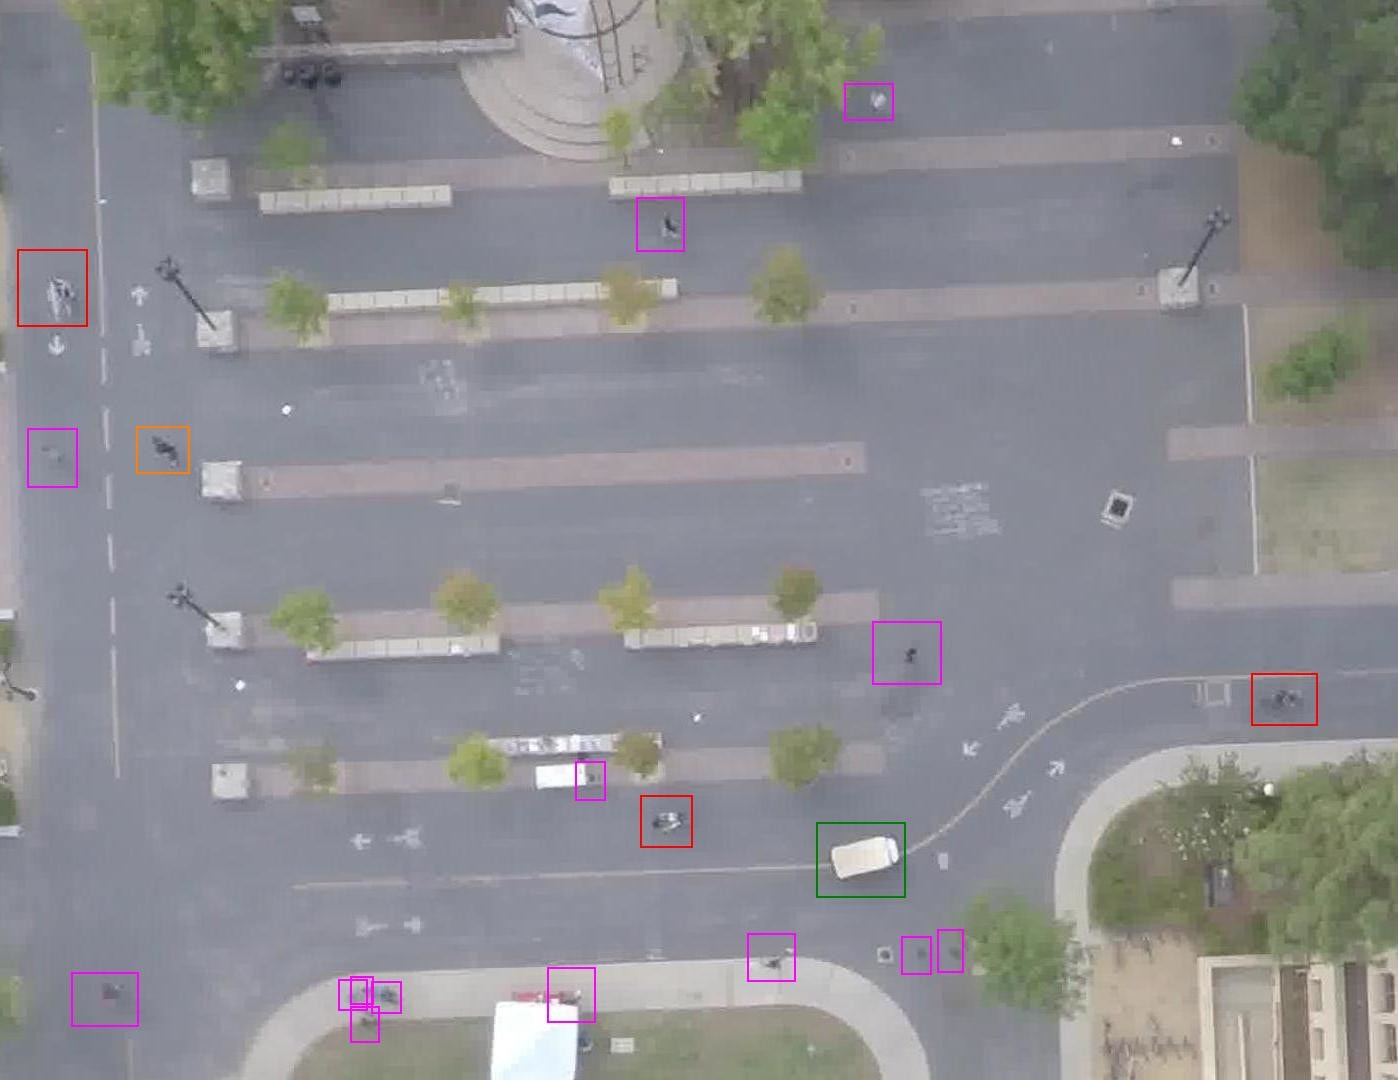
\includegraphics[width=.99\textwidth]{dataset_1.jpg}
    \end{minipage}%
    \begin{minipage}{.5\textwidth}
        \centering
        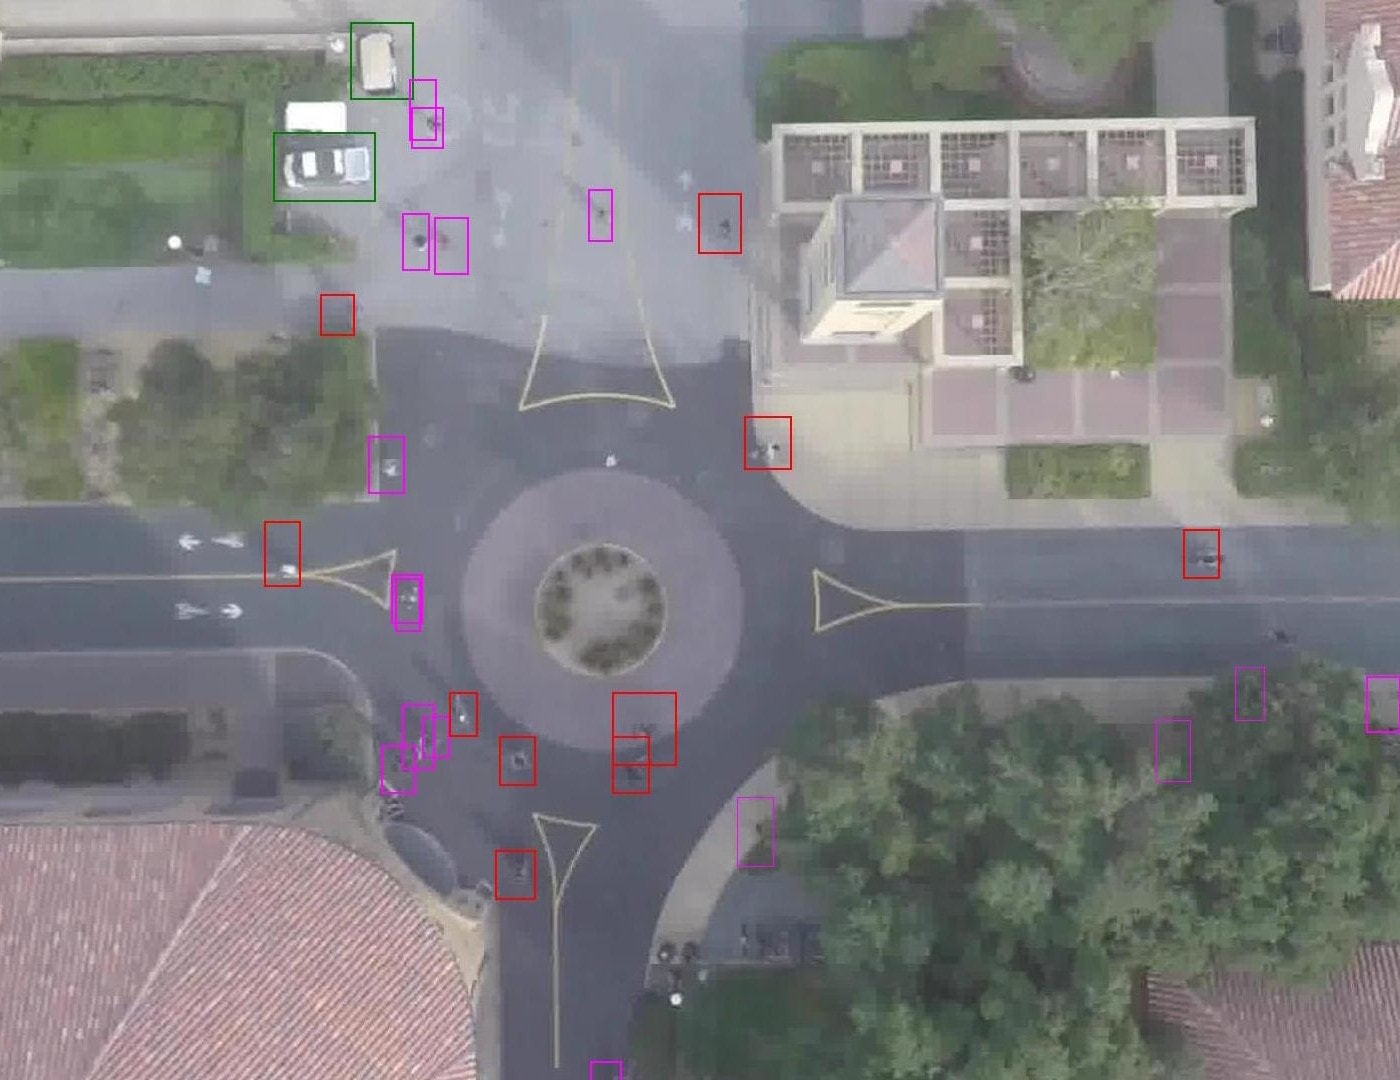
\includegraphics[width=.99\textwidth]{dataset_2.jpg}
    \end{minipage}
    \begin{minipage}{.5\textwidth}
        \centering
        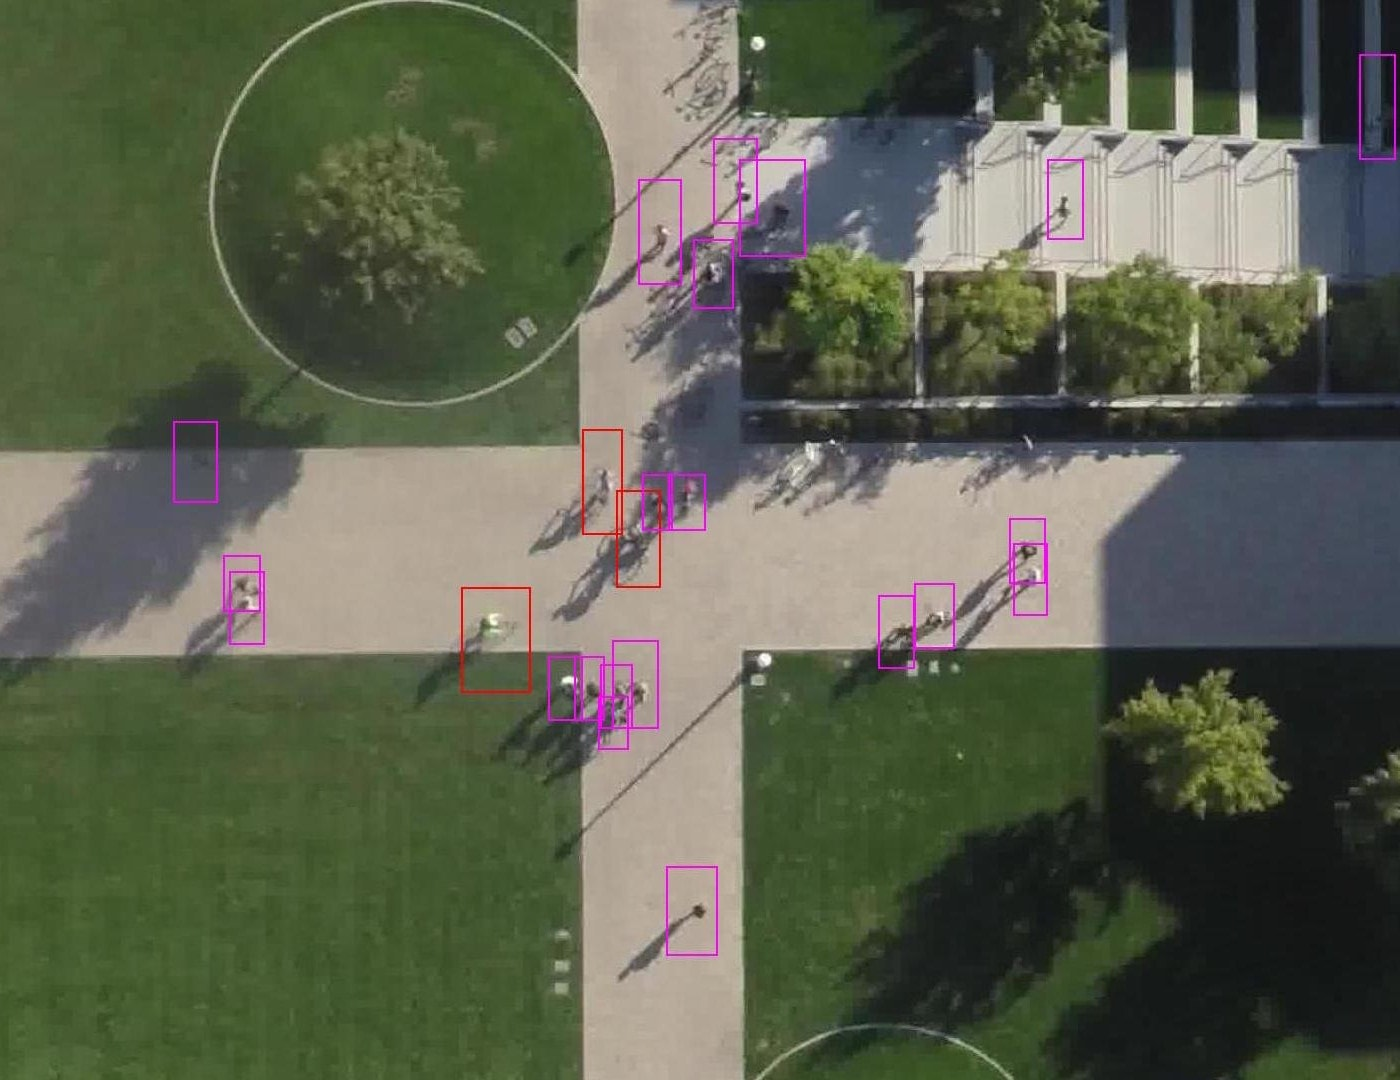
\includegraphics[width=.99\textwidth]{dataset_3.jpg}
    \end{minipage}%
    \begin{minipage}{.5\textwidth}
        \centering
        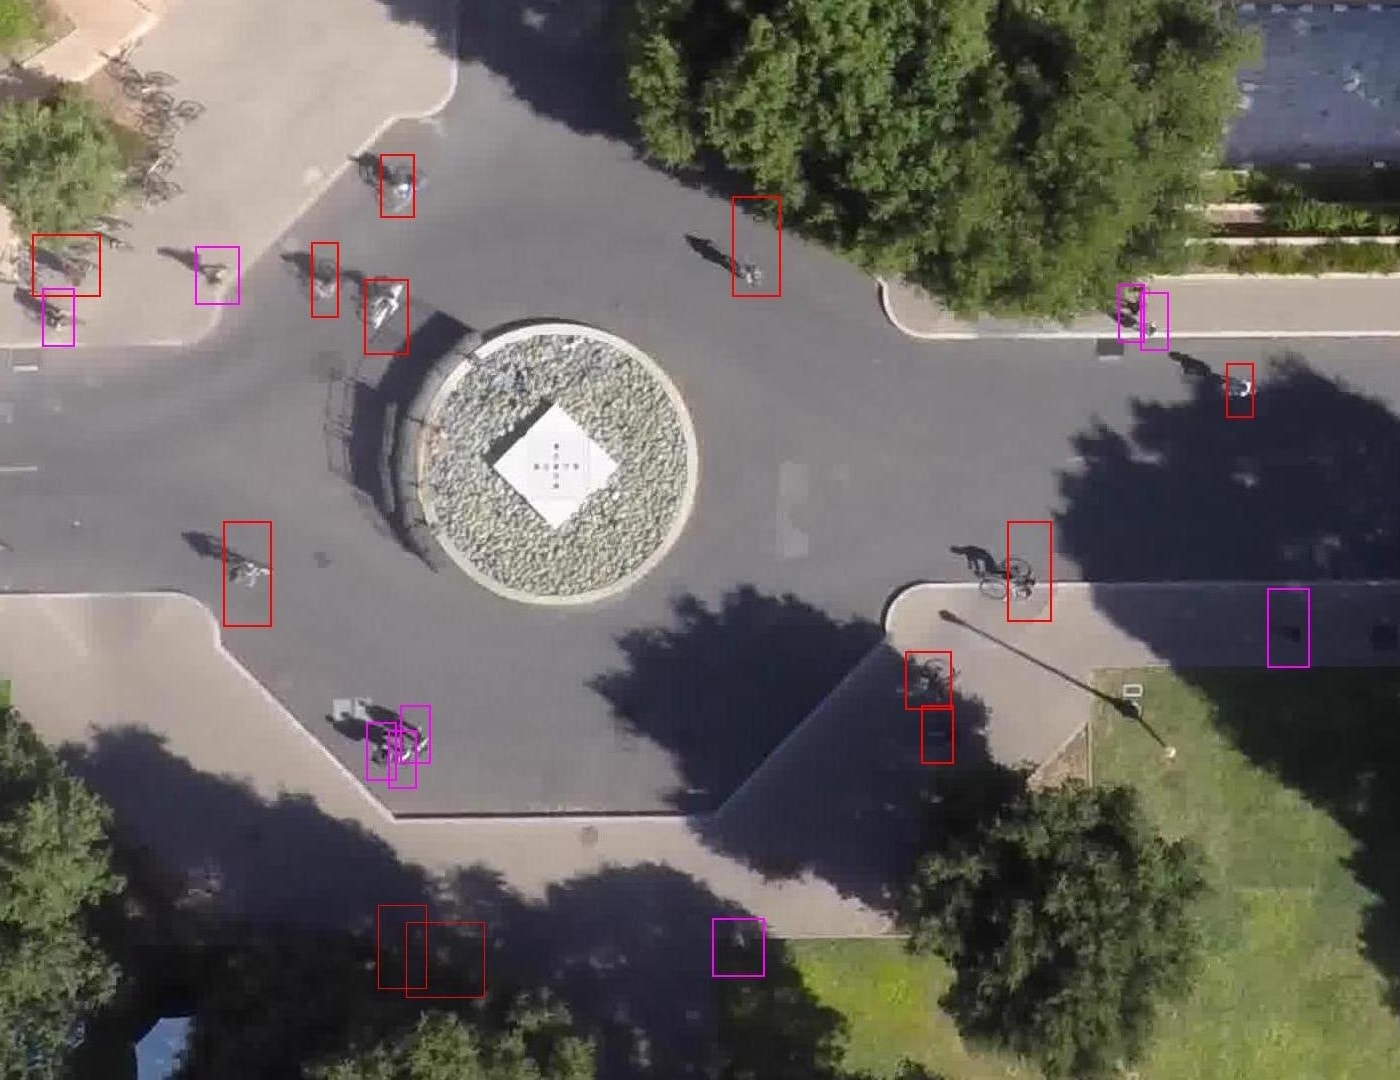
\includegraphics[width=.99\textwidth]{dataset_4.jpg}
    \end{minipage}
    \caption[Ukázka ze datasetu Stanford Drone Dataset]{Ukázka z~použitého datasetu Stanford Drone Dataset.}
\end{figure}

Kvůli syntaxi anotací bylo nutné videozáznamy rozložit po jednotlivých snímcích a upravit informace z~původních anotací do požadovaného formátu. Zároveň pro správné naučení sítě bylo třeba z~anotací vyřadit objekty jiných tříd než chodců a také všechny objekty označené jako \textit{lost} a \textit{occluded}. Veškeré úpravy datasetu probíhaly pomocí skriptů napsaných v~jazyce Python využívajících knihovny OpenCV.

Upravený dataset obsahoval přes 520\,000~obrázků ve formátu jpg o~celkové velikosti 150\,GiB, anotovaných chodců bylo více než~3\,800\,000. Zda anotace opravdu odpovídají konkrétním snímkům, bylo otestováno pomocí debugovacího nástroje \path{retinanet-debug}, který je taktéž součástí použité implementace. Umožňuje vizualizovat anotované objekty~--~označí objekt v~daném snímku podle souřadnic uvedených v~anotaci.

%===============================================================================

\section{Proces trénování}
\label{sec_training_process}

Samotné trénování probíhalo pomocí již zmíněného trénovacího skriptu \path{retinanet-train}. Váhy byly u~každého trénování inicializovány z~předtrénovaného modelu na datasetu ImageNet. To by mělo zajistit rychlejší konvergenci než u~náhodné inicializace. Jako páteřní síť byla zvolena dopředná konvoluční síť ResNet s~50~vrstvami. Byla vybrána příslušná grafická karta a adresář pro ukládání tensorboard statistik z~trénování. U~každého trénovacího snímku byla jistá šance, že se před trénováním otočí, jelikož síť by neměla být zavislá na tom, jak je chodec natočený ke kameře a jakým směrem jde. Každé trénování probíhalo 60~epoch~--~$60\times$~byl síti představen celý dataset. Při trénování neuronové sítě je běžná praxe, že se obrázky síti nepředkládají po jednom, ale po balíčcích (\textit{batches}) určité velikosti (\textit{batch size}). Trénování se poté skládá z~kroků (\textit{steps}), které jsou definovány rovnicí~\ref{eq_steps_definition}.

\begin{equation}
    steps = \frac{velikost \: datasetu}{batch \: size}
    \label{eq_steps_definition}
\end{equation}

Počet kroků byl zvolen na~2\,500, což s~množstvím snímků v~průměru 10\,000 znamená, že síti byly předkládány anotační snímky po zhruba 4~kusech. Dále z~každé scény byly vybrány snímky z~jednoho videa, které sloužily jako validační data. Jednalo se zhruba o~10\,\%~dat. Každé trénování, celých 60~epoch, proběhlo za čas kolem 20~hodin. Veškeré hromadné manipulace a modifikace datasetu probíhaly pomocí skriptů napsaných v~jazyce Python či Bash.

%-------------------------------------------------------------------------------

\subsection*{První trénování}

Po úpravách datasetu zmíněných v~sekci~\ref{sec_dataset} bylo k~dispozici přes 520\,000 obrázků s~3\,800\,000 anotovanými chodci. Snímky jsou však pořízeny z~videa o~30~fps. Dá se předpokládat, že v~průběhu jedné vteřiny, se příliš věcí v~záběru nezmění. Chodci budou posunuti o~pár pixelů dále, ale že by každý snímek přinášel nové relevantní informace o~tom, jak chodec vypadá, je nepravděpodobné. Použití všech snímků by znamenalo pouze prodloužení procesu trénování, protože v~podstatě stejná, či velmi podobná informace by byla zaznamenána na několika snímcích. Proto byl pro trénování použit až každý 50.~snímek. To znamenalo, že pro první učení bylo pro trénování anotováno 67\,386~chodců a pro validaci 9\,907.

\begin{figure}[H]
    \centering
    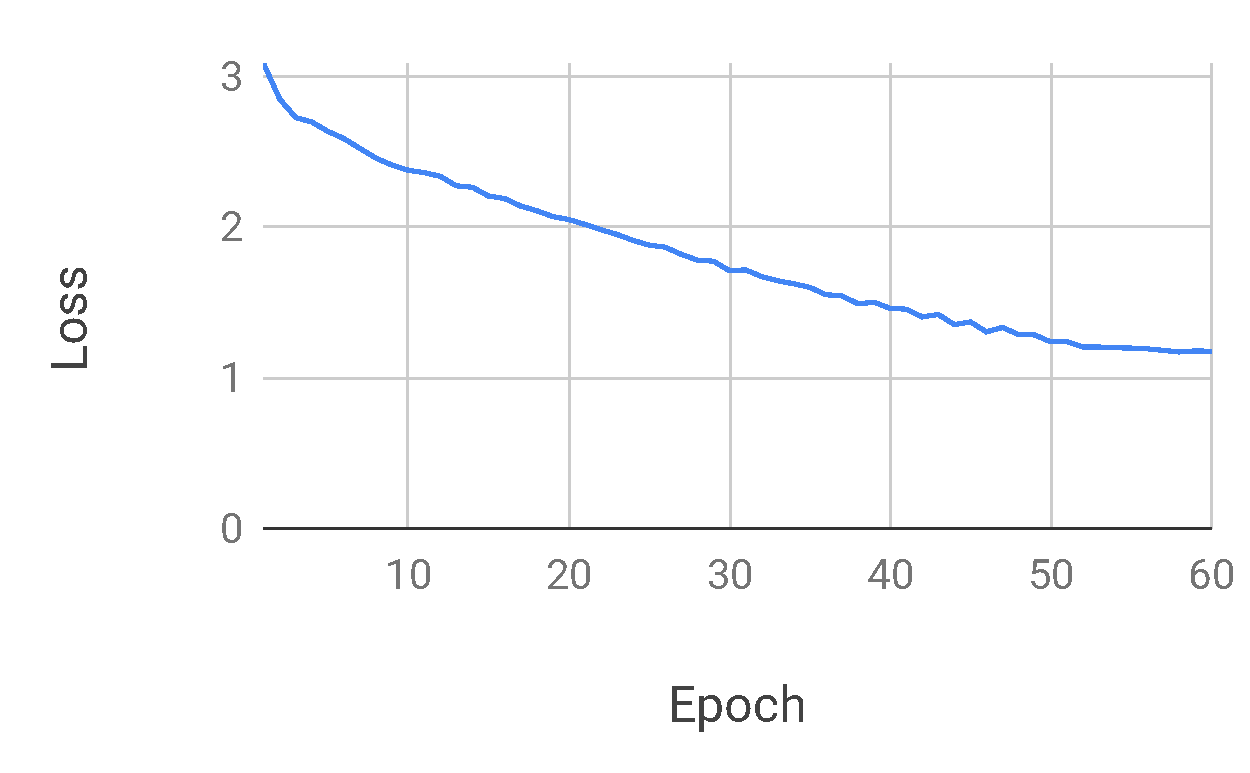
\includegraphics[width=.49\textwidth]{t1-loss.pdf}\hfill
    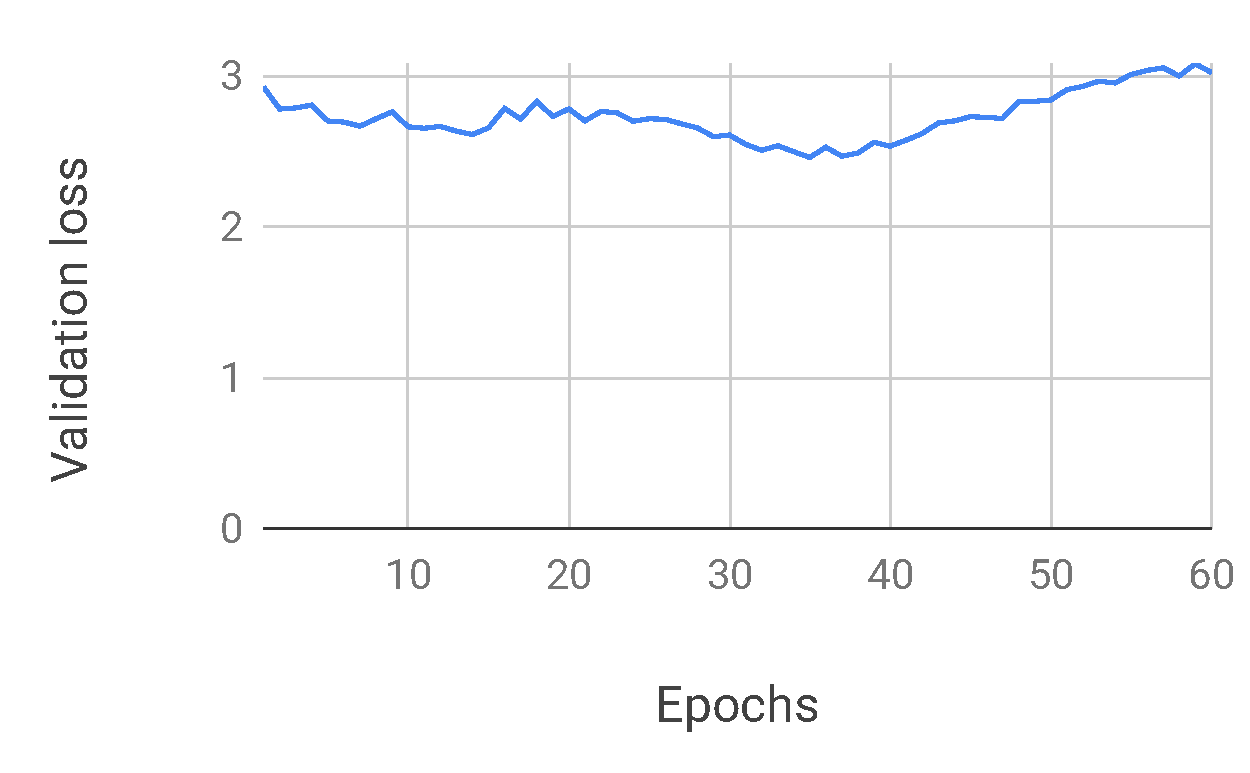
\includegraphics[width=.49\textwidth]{t1-val_loss.pdf}
    \caption[Chyba a validační chyba prvního trénování]{Porovnání chyby a validační chyby modelu z~prvního trénování v~závislosti na množství odtrénovaných epoch.}
    \label{fig_train1_graph}
\end{figure}

Nejlépe si trénovaný model vedl kolem 35.~epochy, potom validační chyba začala růst a model začal jevit známky přetrénování. Z~podrobnějšího prozkoumání a otestování výsledků prvního trénování vyplynulo, že spousta cyklistů je mylně rozpoznáno jako chodci a spousta chodců zase jako cyklisti. V~původním datasetu tvořili anotovaní chodci zhruba~45\,\% a cyklisté~40\,\%. Z~výšky je velmi těžké, někdy až nemožné rozeznat co je cyklista a co chodec. Na snímcích je zachycena spousta cyklistů, kteří vypadají jako chodci. Tyto anotace síť mátly a to byl jeden z~důvodů vysoké validační chyby a nepřesnosti modelu.

\begin{figure}[H]
    \centering
    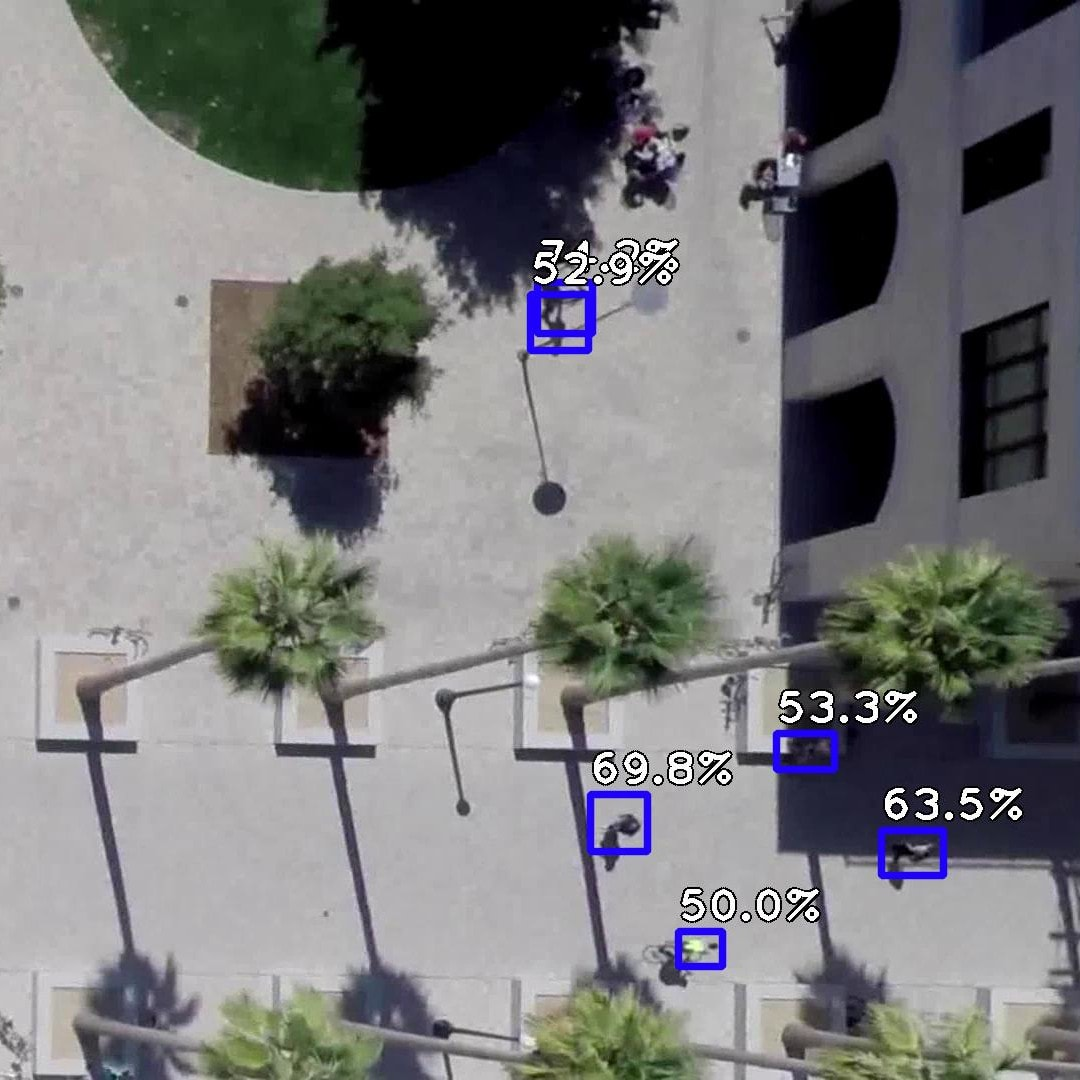
\includegraphics[width=.33\textwidth]{t1-v1.jpg}\hfill
    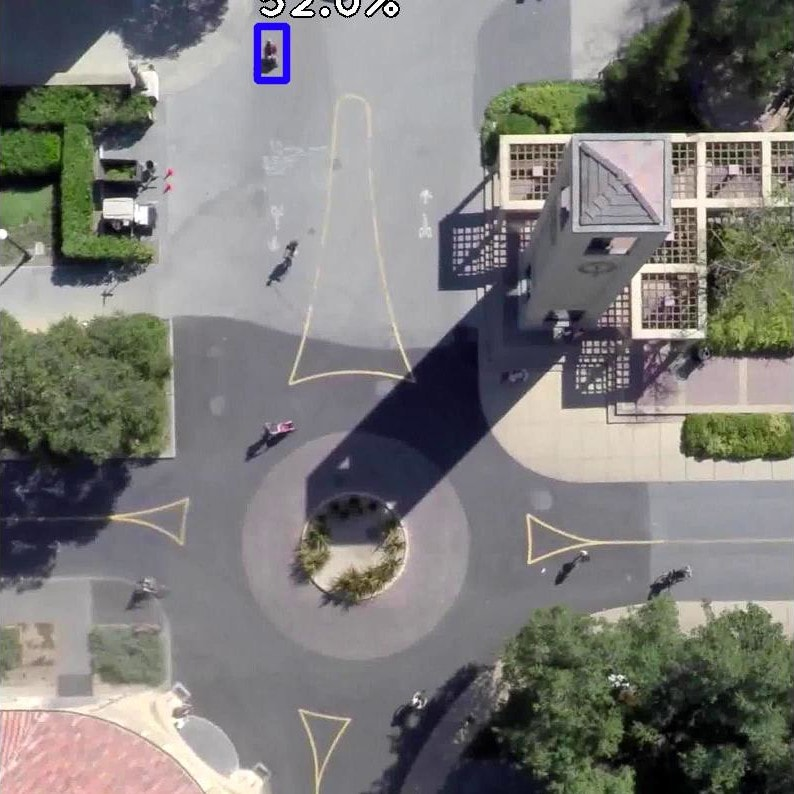
\includegraphics[width=.33\textwidth]{t1-v2.jpg}\hfill
    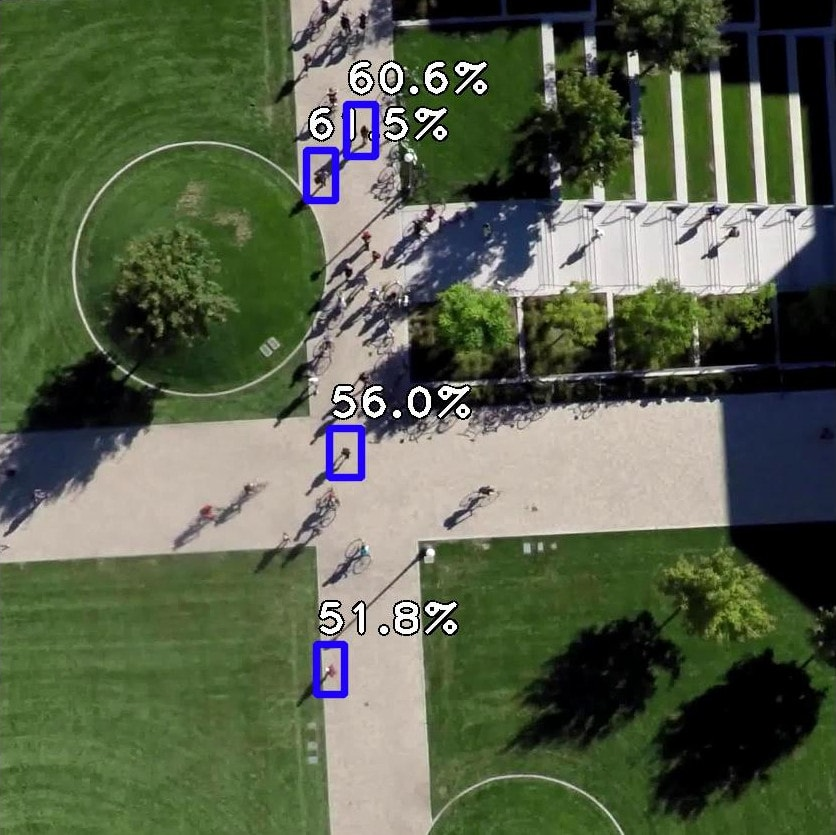
\includegraphics[width=.33\textwidth]{t1-v3.jpg}
    \caption[Validace modelu z~prvního trénování na validačních snímcích]{Validace modelu z~prvního trénování na validačních snímcích.}
    \label{fig_train1_val_img}
\end{figure}

\begin{figure}[H]
    \centering
    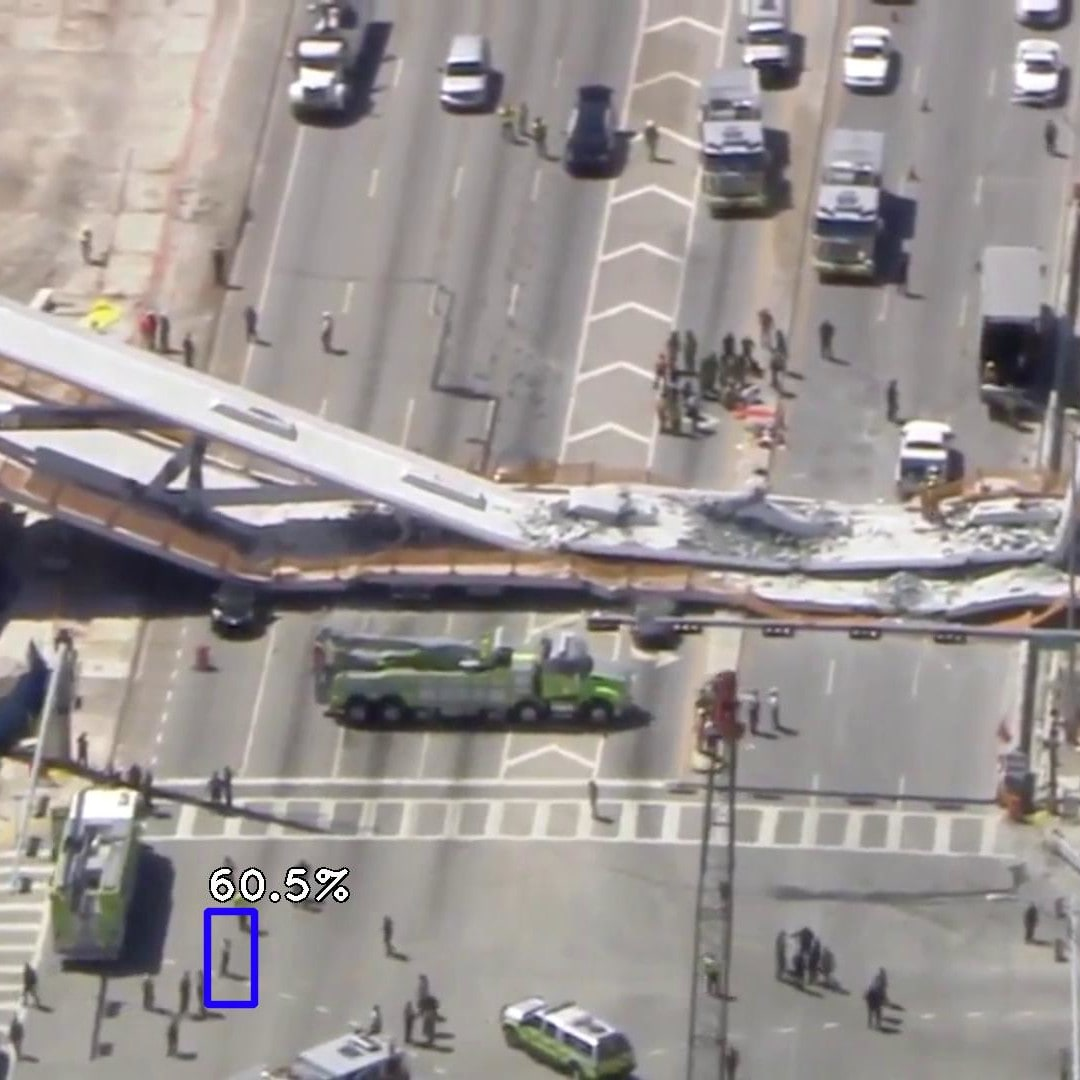
\includegraphics[width=.33\textwidth]{t1-t1.jpg}\hfill
    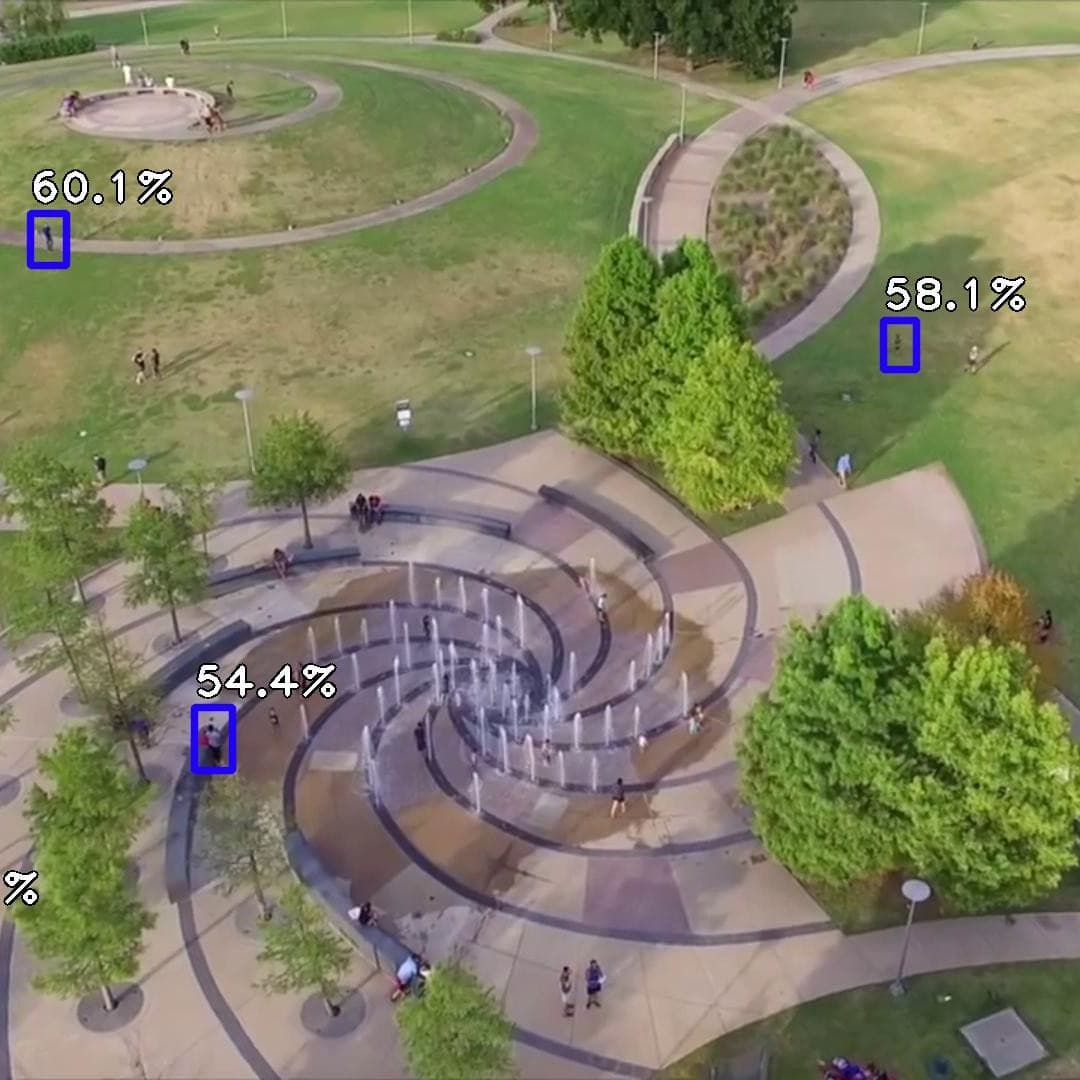
\includegraphics[width=.33\textwidth]{t1-t2.jpg}\hfill
    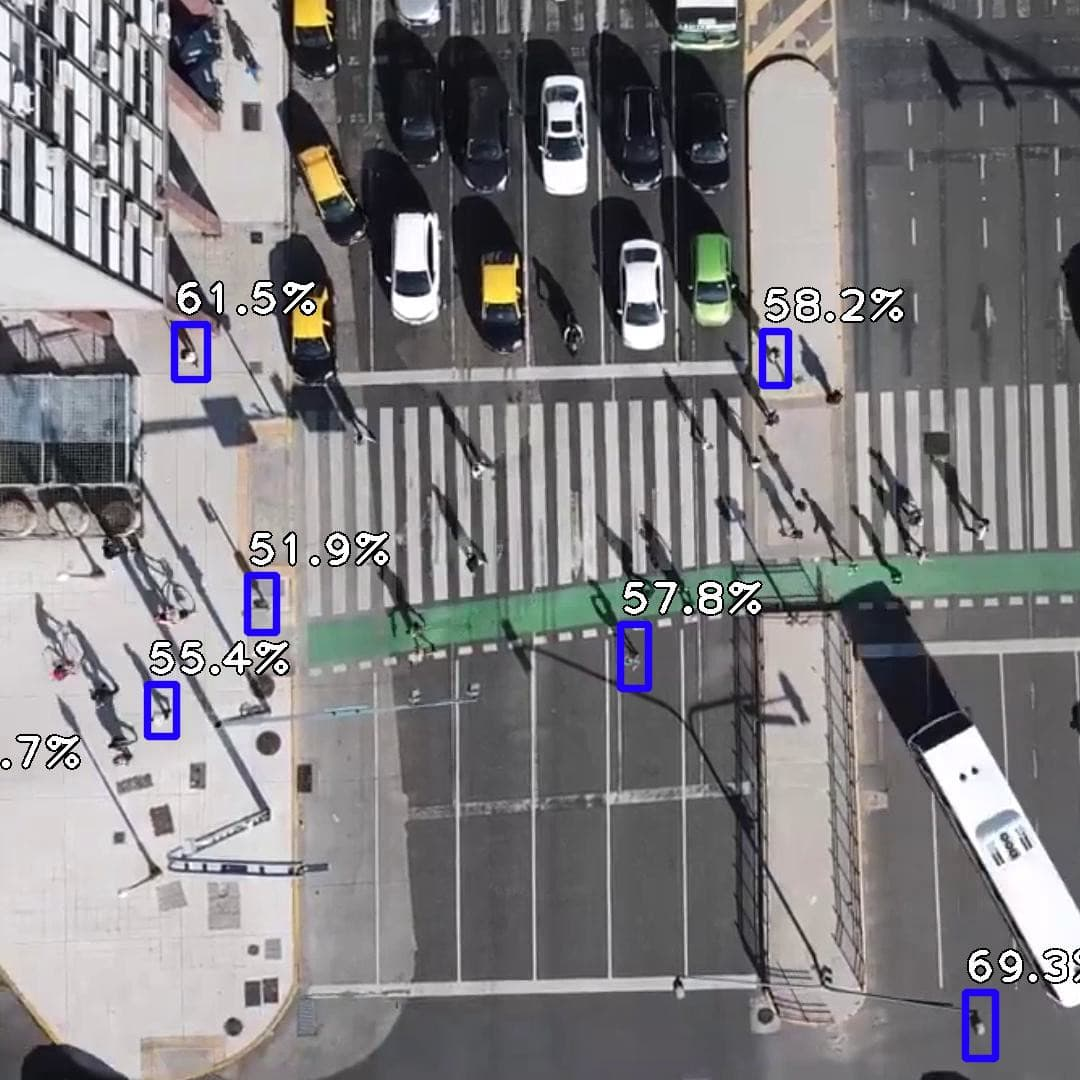
\includegraphics[width=.33\textwidth]{t1-t3.jpg}
    \caption[Validace modelu z~prvního trénování na testovacích snímcích]{Validace modelu z~prvního trénování na testovacích snímcích, které nebyly součástí původního datasetu.}
    \label{fig_train1_test_img}
\end{figure}

%-------------------------------------------------------------------------------

\subsection*{Druhé trénování}

Na základě poznatků z~prvního trénování byl dataset pro další trénování upraven. Do anotací byli zahrnuti nejen chodci, ale také cyklisté a lidé na skateboardu. To vše pod jednou společnou třídou.

Druhá úprava spočívala v~úpravě počtu snímků z~jednotlivých scén. Videa z~některých scén byla výrazně kratší, či obsahovala výrazně odlišný počet anotací. To mohlo mít za následek, že některé typy záběrů byly sítí preferovány. Například z~určité výšky, z~určitého úhlu či daného barevného spektra ovlivněné světelnými podmínkami ve scéně. Proto pro další trénování nebyl vybrán každý 50.~snímek z~každé scény, ale snímkování bylo ovlivněno počtem anotací z~jednotlivých scén. A~to tak, aby každá scéna obsahovala zhruba stejný počet anotací. Pro druhé učení bylo trénovacích anotací 55\,241 a validačních 8\,263.

\begin{figure}[H]
    \centering
    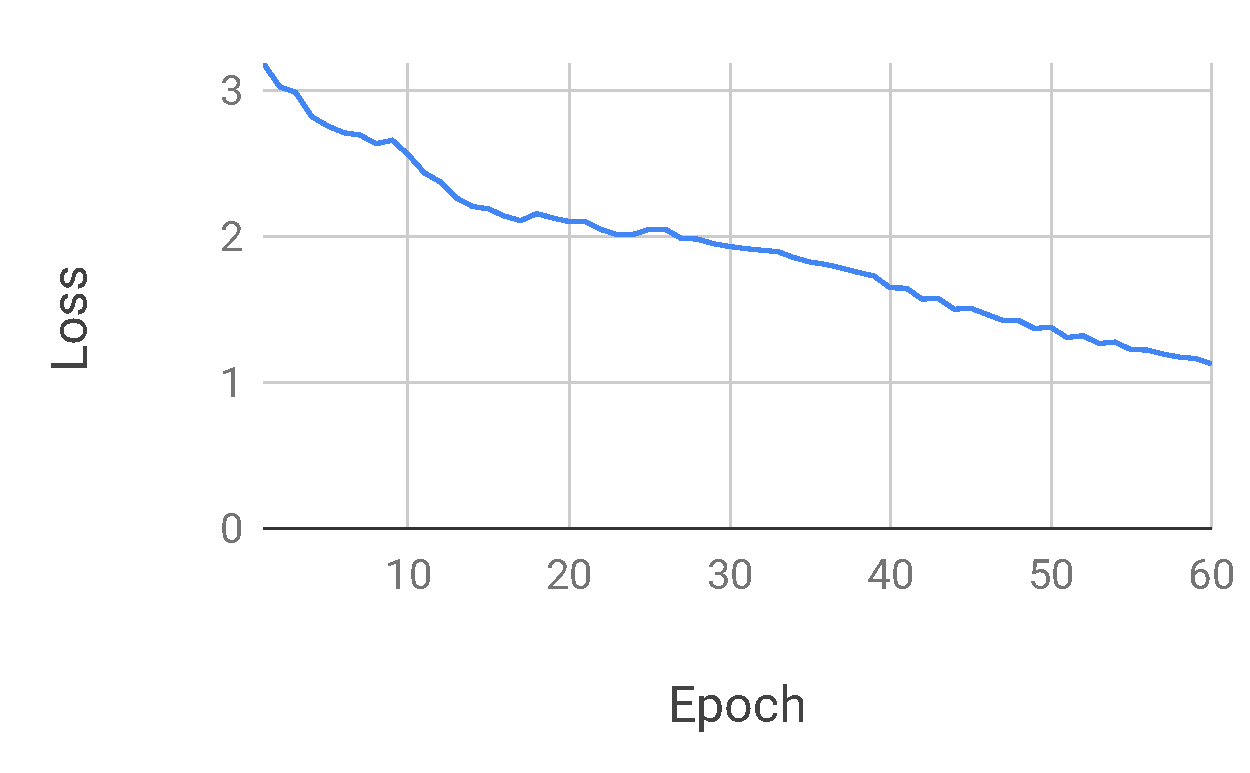
\includegraphics[width=.49\textwidth]{t2-loss.pdf}\hfill
    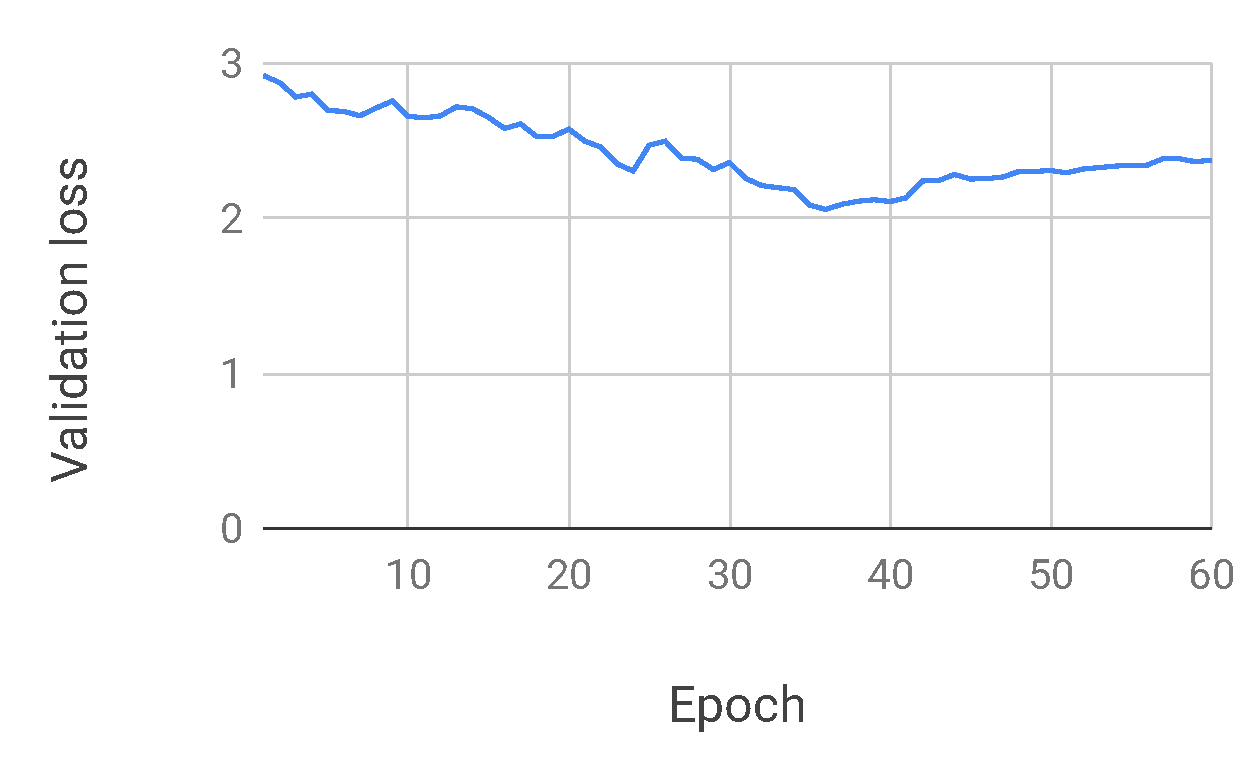
\includegraphics[width=.49\textwidth]{t2-val_loss.pdf}
    \caption[Chyba a validační chyba druhého trénování]{Porovnání chyby a validační chyby modelu z~druhého trénování v~závislosti na množství odtrénovaných epoch.}
    \label{fig_train2_graph}
\end{figure}

Jako u~prvního trénování si model nejlépe vedl kolem 35.~epochy. Výsledky byly lepší, ale ne uspokojivé. Dalším zkoumáním bylo zjištěno, že spousta anotací je uvedena úplně mylně. Například příznaky \textit{occluded} nebyly uvedeny ve 100\,\%~případech, a tak v~anotacích byla spousta anotovaných objektů například pod stromem či pod střechou domu. Jindy byly zase anotace úplně mimo objekt nebo objekt pokrývaly jen zčásti. Tyto neduhy datasetu byly pravděpodobně způsobeny skutečností, s~jakým účelem byl dataset vytvářen -- predikce pohybů objektů. V~takovém případě není důležité, zda je chodec na kameře skutečně vidět, je skrytý pod stromem nebo zda je anotován pouze zčásti. Bohužel chybných anotací bylo poměrně velké množství a pro lepší a přesnější výsledky bude nutné dataset ručně projít a obrázky s~chybnými anotacemi vymazat.

\begin{figure}[H]
    \centering
    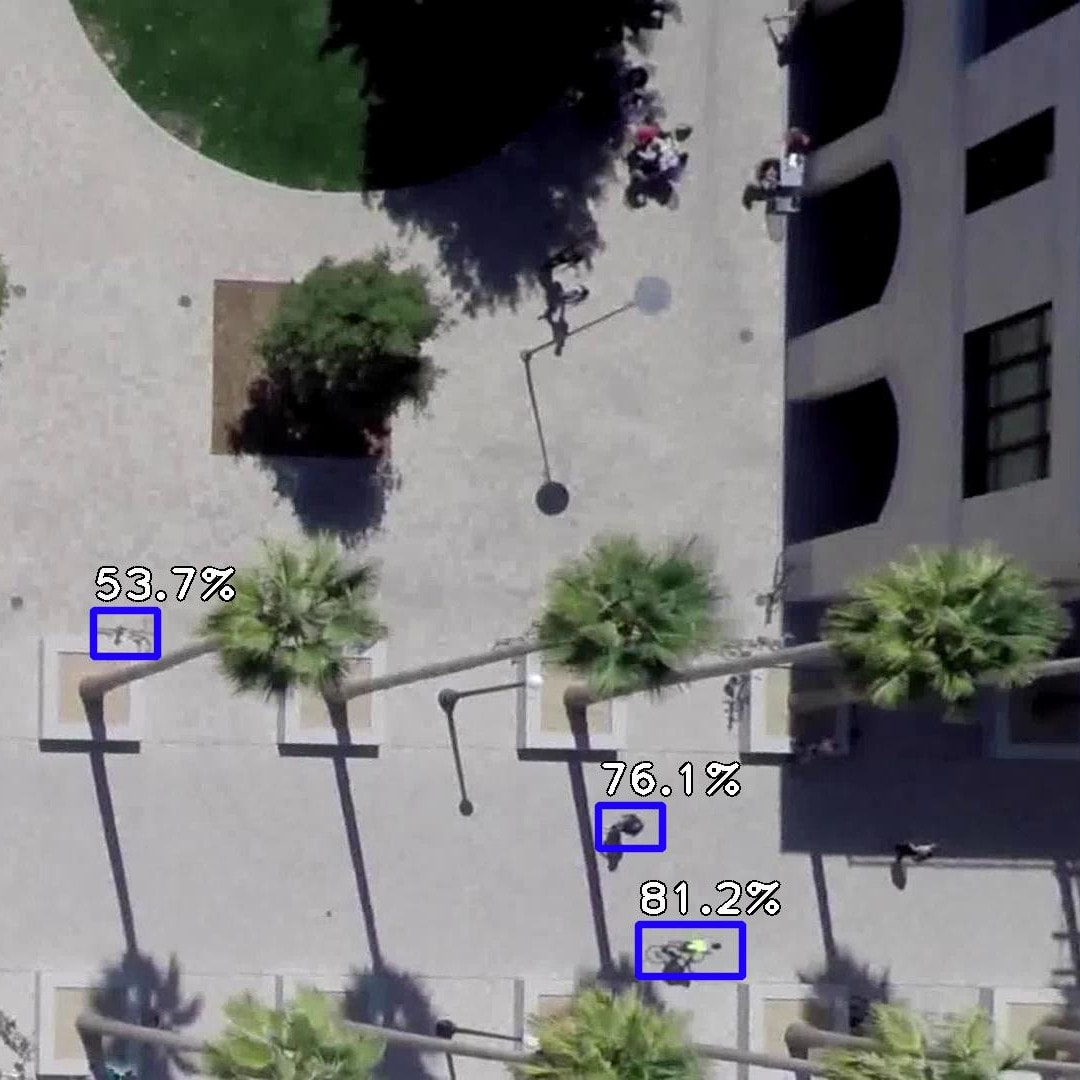
\includegraphics[width=.33\textwidth]{t2-v1.jpg}\hfill
    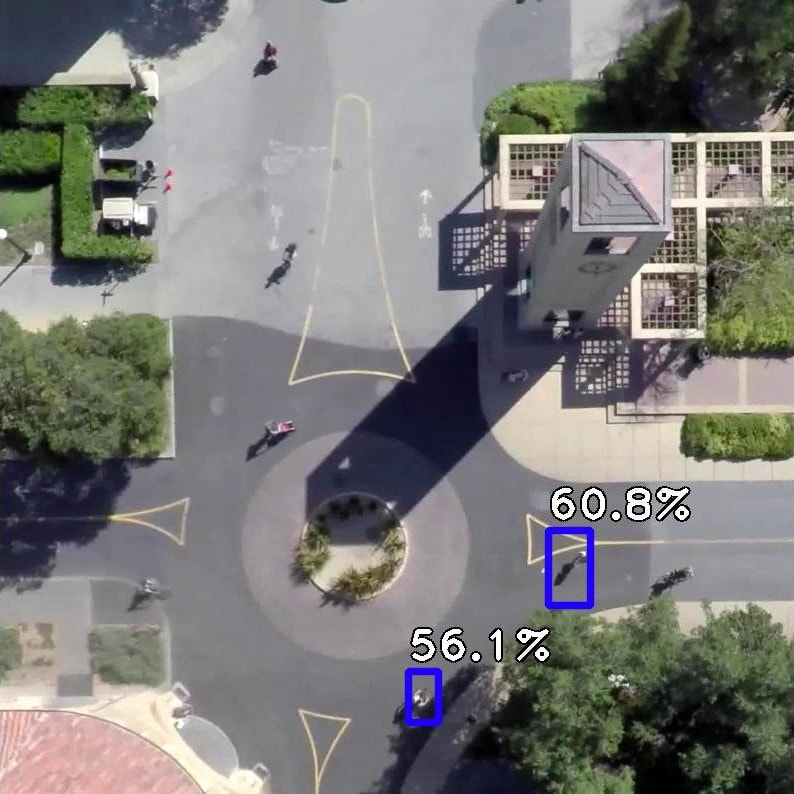
\includegraphics[width=.33\textwidth]{t2-v2.jpg}\hfill
    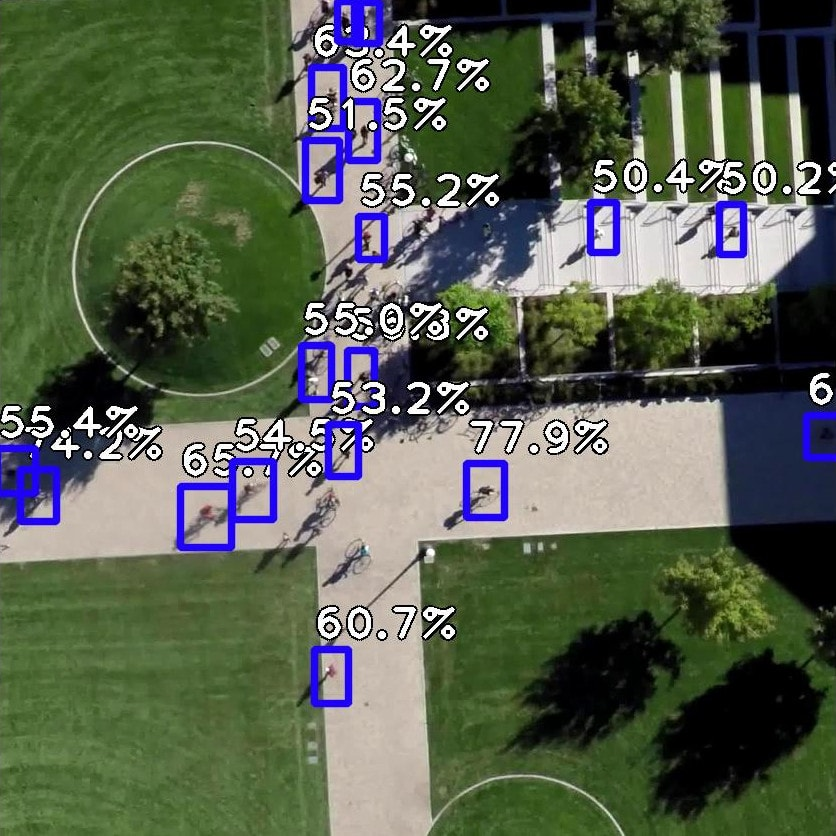
\includegraphics[width=.33\textwidth]{t2-v3.jpg}
    \caption[Validace modelu z~druhého trénování na validačních snímcích]{Validace modelu z~druhého trénování na validačních snímcích.}
    \label{fig_train2_val_img}
\end{figure}

\begin{figure}[H]
    \centering
    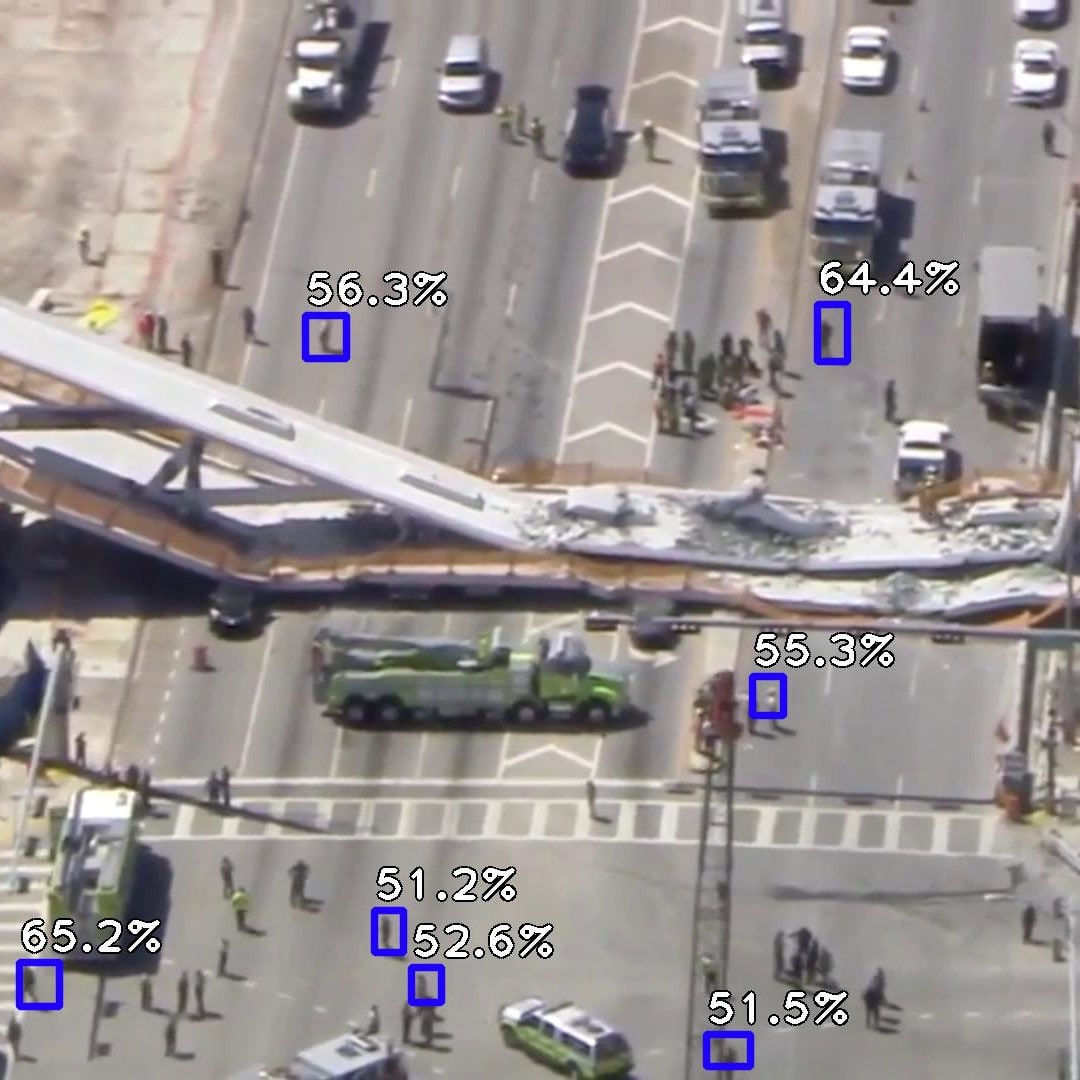
\includegraphics[width=.33\textwidth]{t2-t1.jpg}\hfill
    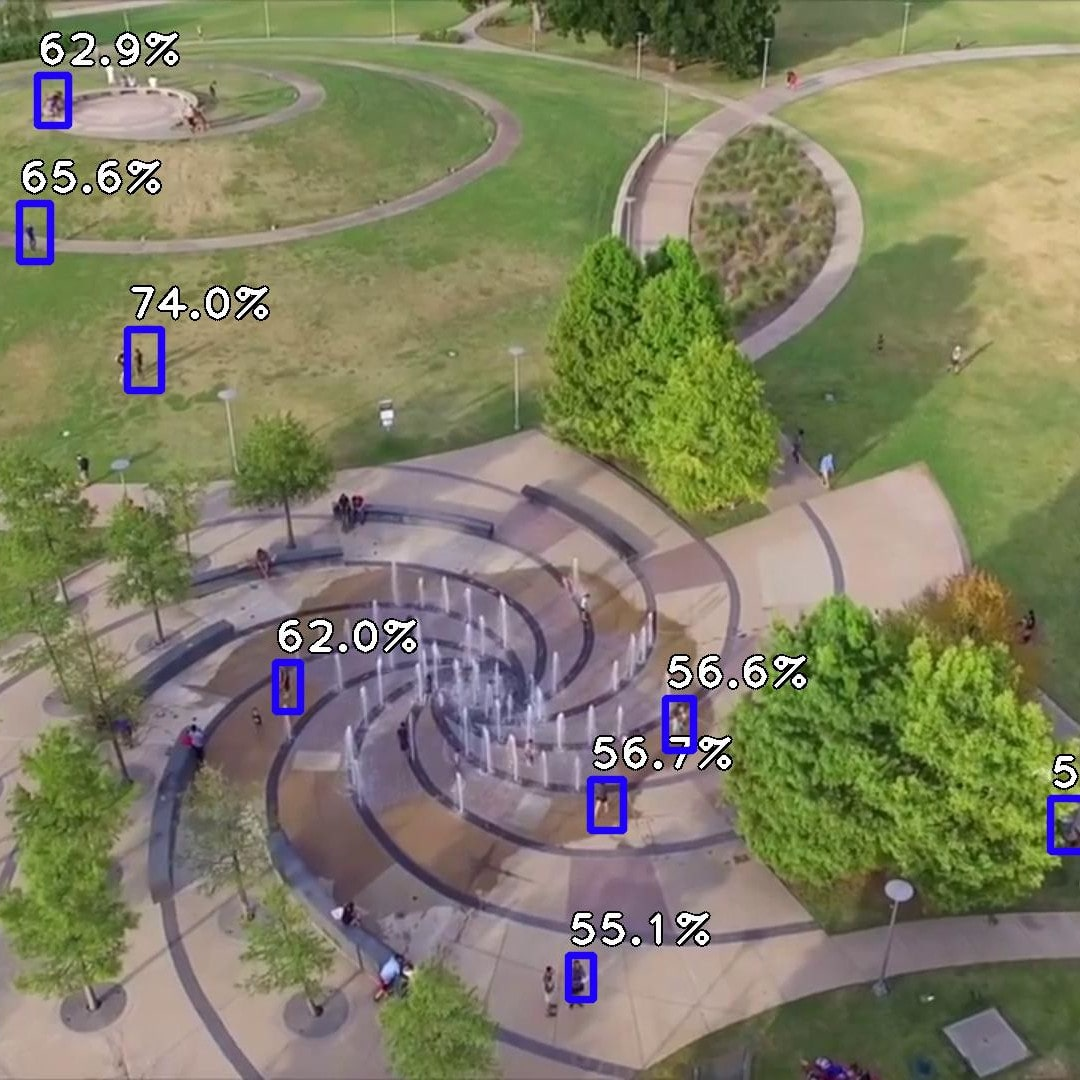
\includegraphics[width=.33\textwidth]{t2-t2.jpg}\hfill
    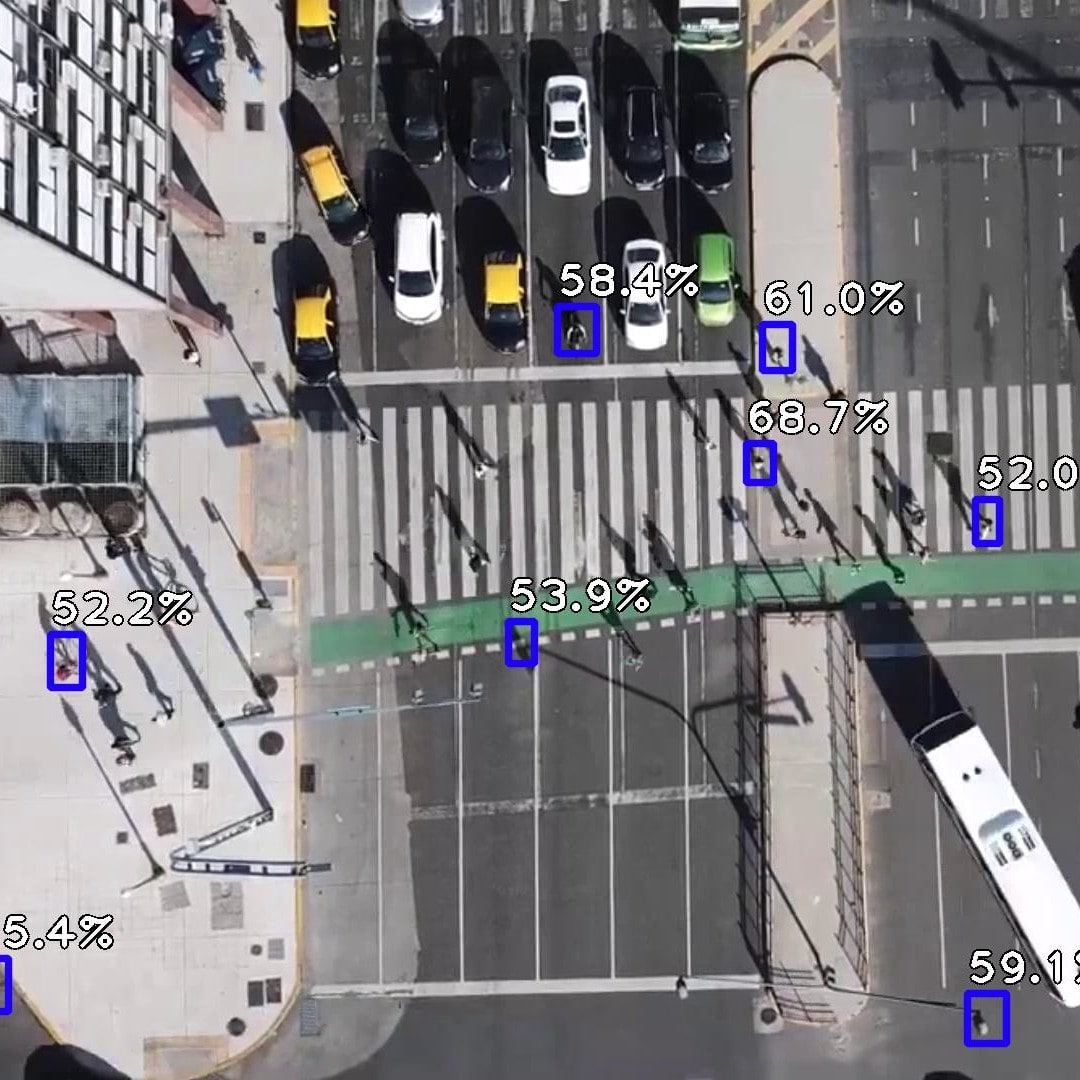
\includegraphics[width=.33\textwidth]{t2-t3.jpg}
    \caption[Validace modelu z~druhého trénování na testovacích snímcích]{Validace modelu z~druhého trénování na testovacích snímcích, které nebyly součástí původního datasetu.}
    \label{fig_train2_test_img}
\end{figure}

%-------------------------------------------------------------------------------

\subsection*{Třetí trénování}

Pro třetí trénování byl dataset ručně protřízen. Pomocí skriptu \path{retinanet-evaluate}, který je součástí použité implementace RetinaNet, byly vykresleny anotace přímo do příslušných snímků. Poté byly ručně zkontrolovány a ty, kde byly anotace nepřesné či úplně chybné, byly vyřazeny. Celkově bylo vymazáno 1\,926~snímků z~9\,549~vygerovaných stejným způsobem jako u~druhého trénování, aby anotace z~žádné scény nepřevažovaly. Anotací pro trénování zůstalo 63\,433 a anotací pro validaci 14\,010.

\begin{figure}[H]
    \centering
    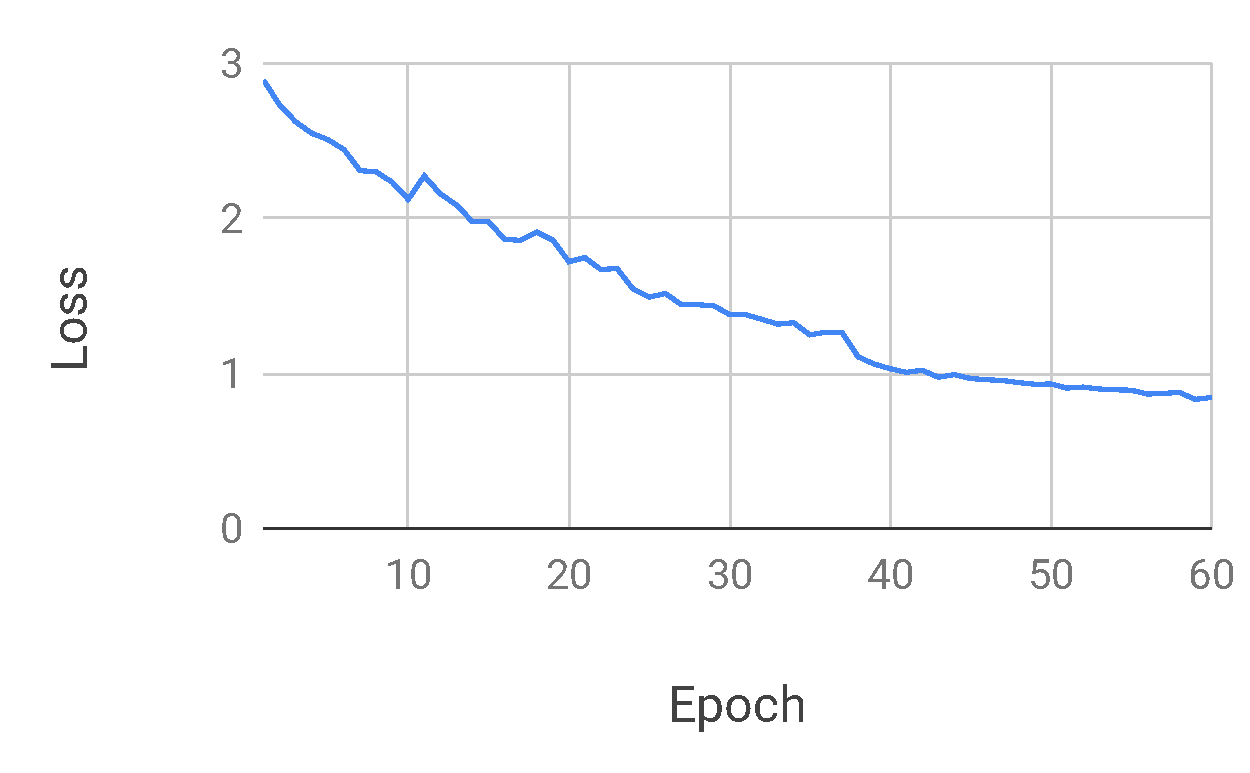
\includegraphics[width=.49\textwidth]{t3-loss.pdf}\hfill
    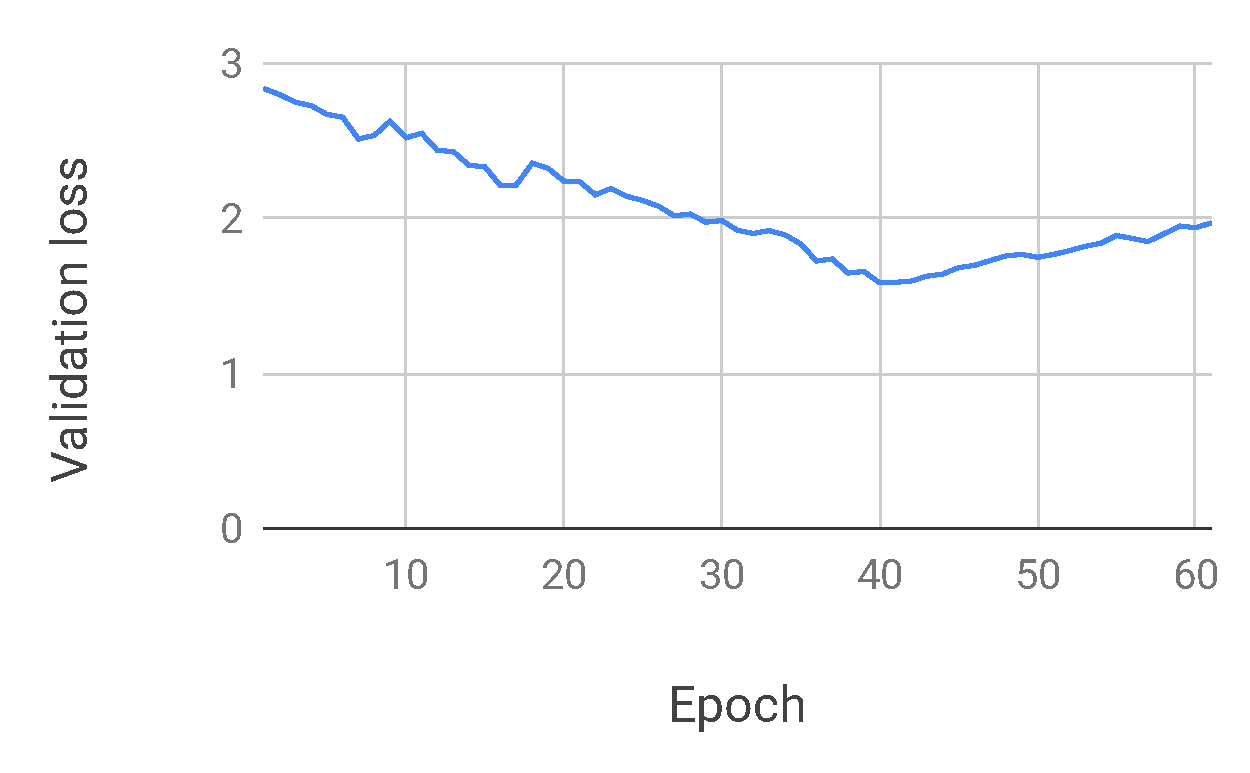
\includegraphics[width=.49\textwidth]{t3-val_loss.pdf}
    \caption[Chyba a validační chyba třetího trénování]{Porovnání chyby a validační chyby modelu z~třetího trénování v~závislosti na množství odtrénovaných epoch.}
    \label{fig_train3_graph}
\end{figure}

Model tentokrát dosáhl nejlepších výsledků kolem 40.~epochy, ty byly opět lepší než v~předchozím trénování. Validační chyba dosáhla minimální hodnoty 1,58. Tyto výsledky již považuji vzhledem k~výpočetním možnostem a rozmanitosti datasetu za dostačující.

\begin{figure}[H]
    \centering
    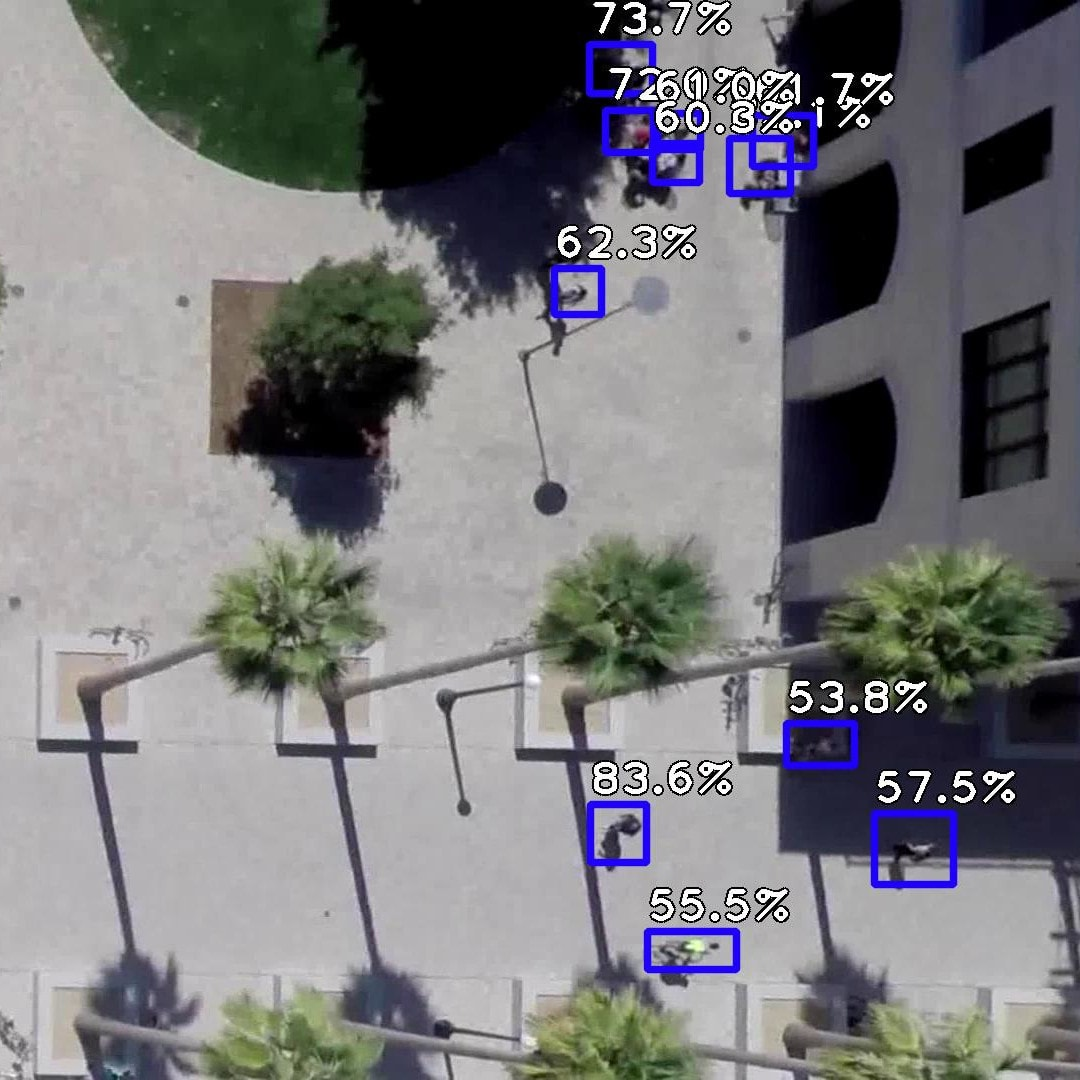
\includegraphics[width=.33\textwidth]{t3-v1.jpg}\hfill
    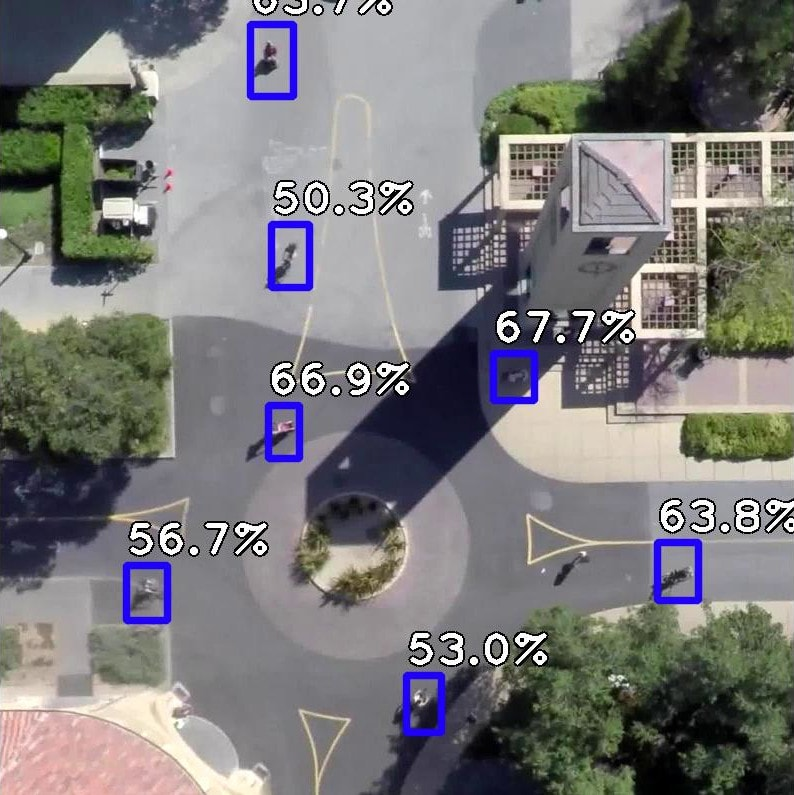
\includegraphics[width=.33\textwidth]{t3-v2.jpg}\hfill
    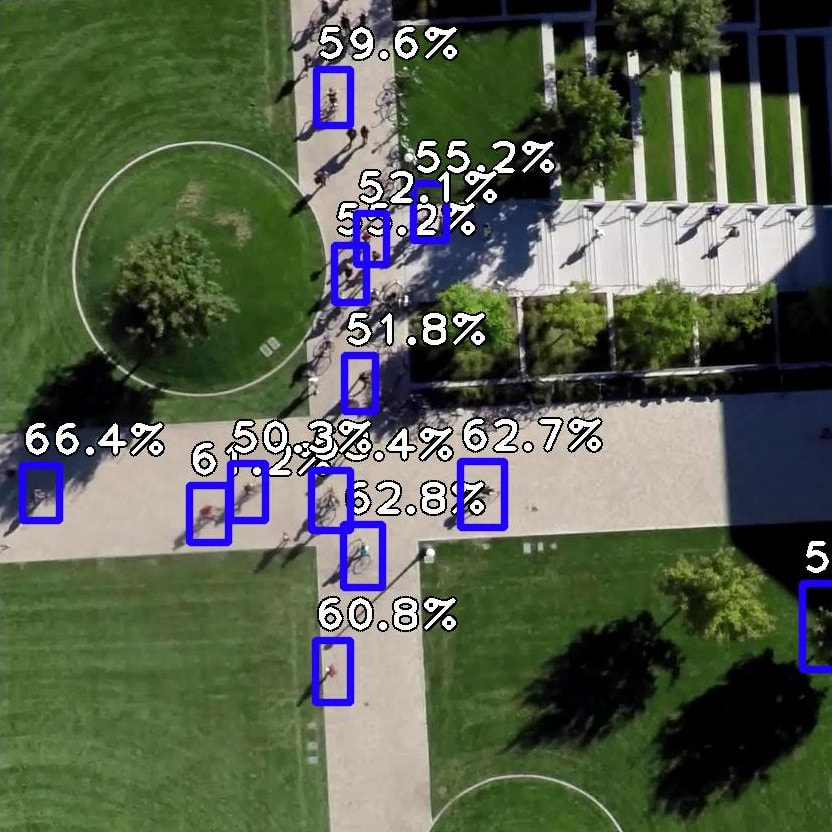
\includegraphics[width=.33\textwidth]{t3-v3.jpg}
    \caption[Validace modelu z~třetího trénování na validačních snímcích]{Validace modelu z~třetího trénování na validačních snímcích.}
    \label{fig_train3_val_img}
\end{figure}

\begin{figure}[H]
    \centering
    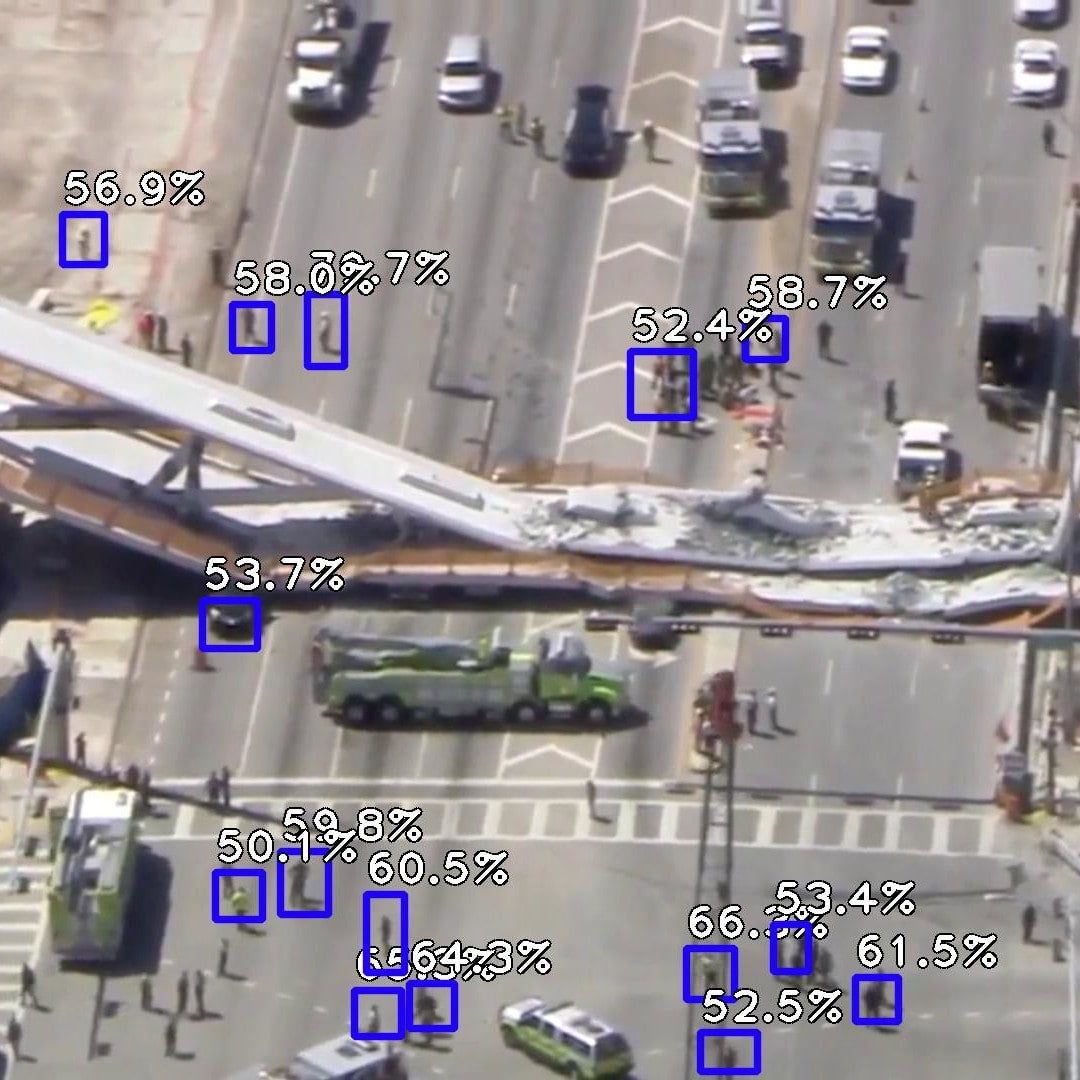
\includegraphics[width=.33\textwidth]{t3-t1.jpg}\hfill
    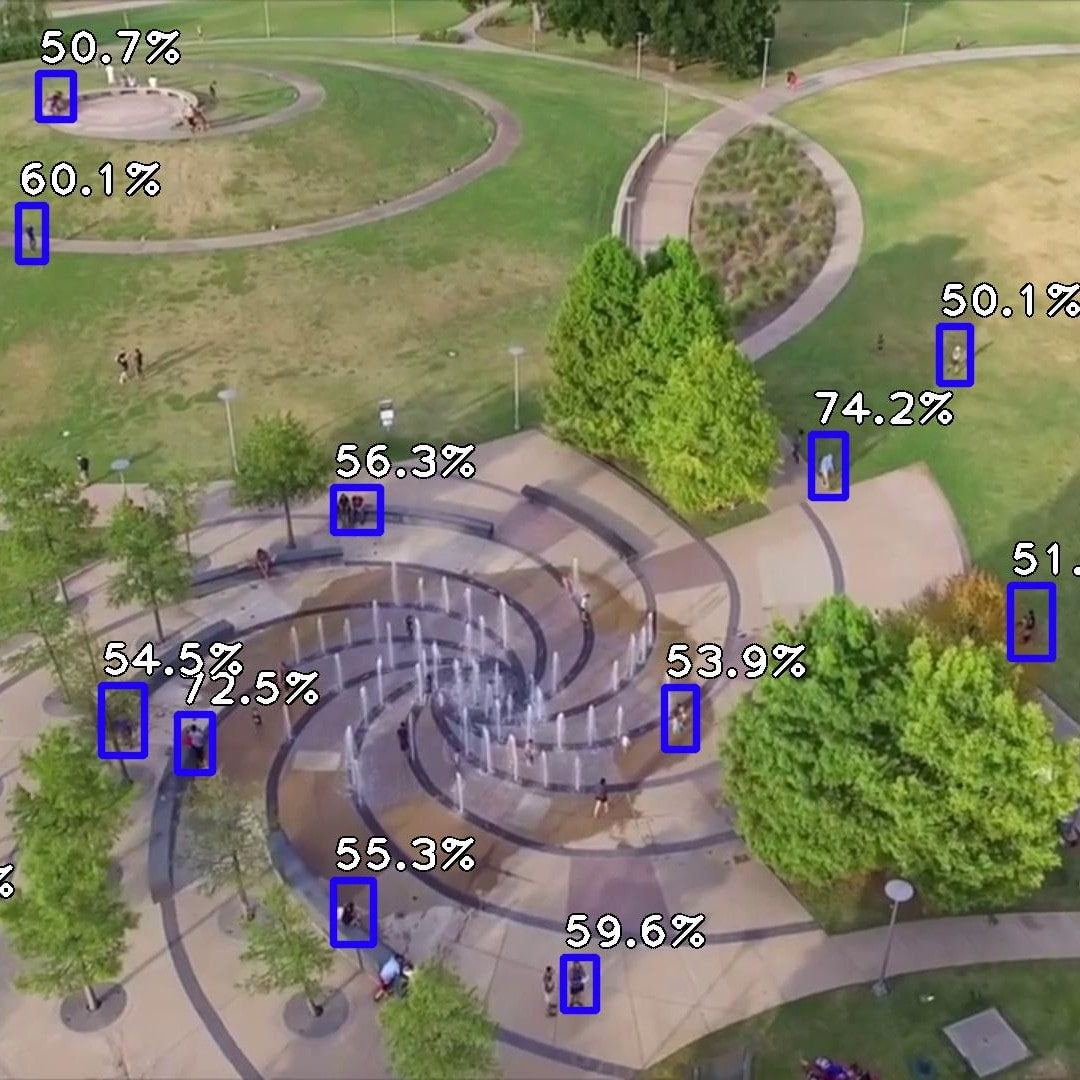
\includegraphics[width=.33\textwidth]{t3-t2.jpg}\hfill
    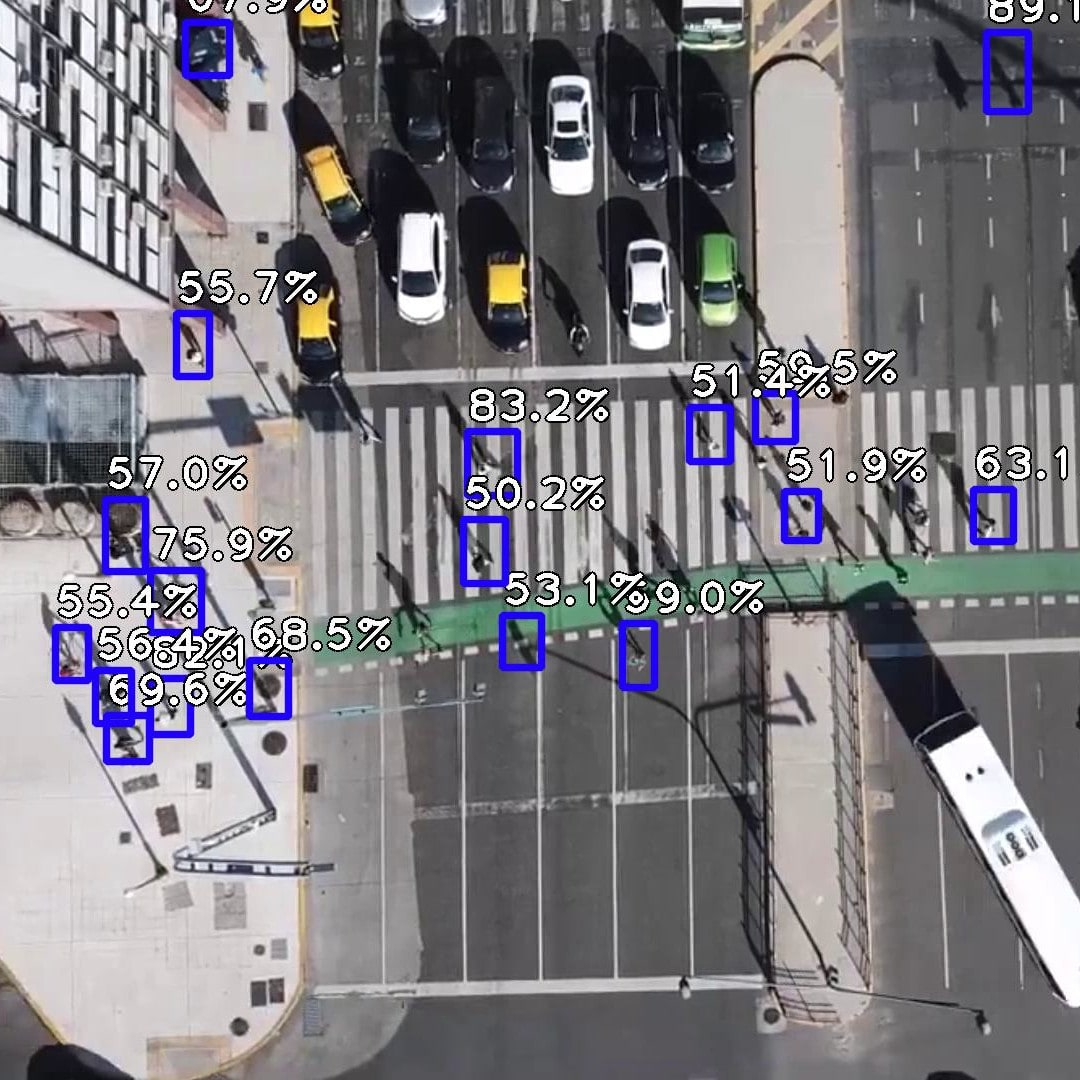
\includegraphics[width=.33\textwidth]{t3-t3.jpg}
    \caption[Validace modelu z~třetího trénování na testovacích snímcích]{Validace modelu z~třetího trénování na testovacích snímcích, které nebyly součástí původního datasetu.}
    \label{fig_train3_test_img}
\end{figure}

%===============================================================================
